\chapter{Extended Examples\label{examples_CHPTEXAMPLES}}
\label{examples_g151}
\label{examples_h0}
\begin{figure}[H]
\centering
\setlength{\fboxrule}{3pt}
\fbox{
\includegraphics[width=0.9\textwidth]{canned/ch12.png}
\begin{rotate}{90}
\copyright~2009 Jean-Pierre H\'{e}bert
\end{rotate}}
\end{figure}
\clearpage





\label{examples_s0}This chapter presents a series of programs
that perform more complicated tasks than most of the examples
found throughout the earlier chapters of the book.
They illustrate a variety of programming techniques and demonstrate a
particular programming style.


Each section of this chapter describes one program in detail and gives
examples of its use.
This is followed by a listing of the code.
At the end of each section are exercises intended to stimulate thought
about the program and to suggest possible extensions.
These exercises are generally more difficult than those found in
Chapters \ref{start_g4} and \ref{further_g49}, and a few
are major projects.


Section \ref{examples_g152} presents a simple matrix multiplication
package.
It demonstrates a set of procedures that could be written in almost any
language.
Its most interesting features are that all multiplication operations
are performed by calling a single \textit{generic} procedure,
\texttt{mul}, which calls the appropriate help procedure depending upon
the dimensions of its arguments, and that it dynamically allocates
results of the proper size.
Section \ref{examples_g158} presents a merge sorting
algorithm for ordering lists according to arbitrary predicates.
Section \ref{examples_g162} describes a syntactic form that is used to
construct sets.
It demonstrates a simple but efficient syntactic transformation from
set notation to Scheme code.
Section \ref{examples_g169} presents a word-counting program borrowed
from \textit{The C Programming Language} [\hyperref[bibliography_g237]{19}], translated
from C into Scheme.
It shows character and string manipulation, data structure creation and
manipulation, and basic file input and output.
Section \ref{examples_g176} presents a Scheme printer that implements
basic versions of \texttt{put-datum}, \texttt{write}, and
\texttt{display}.
Section \ref{examples_g180} presents a simple formatted output facility
similar to those found in many Scheme systems and in other languages.
Section \ref{examples_g187} presents a simple interpreter for
Scheme that illustrates Scheme as a language implementation vehicle while
giving an informal operational semantics for Scheme as well as a useful
basis for investigating extensions to Scheme.
Section \ref{examples_g193} presents a small, extensible abstract
object facility that could serve as the basis for an entire
object-oriented subsystem.
Section \ref{examples_g198} presents a recursive algorithm for computing
the Fourier transform of a sequence of input values.
It highlights the use of Scheme's complex arithmetic.
Section \ref{examples_g204} presents a concise unification algorithm
that shows how procedures can be used as continuations and as
substitutions (unifiers) in Scheme.
Section \ref{examples_g208} describes a multitasking facility and its
implementation in terms of continuations.



\section{\label{examples_g152}\label{examples_h1}Matrix and Vector Multiplication\label{examples_SECTEXMATMUL}}



\label{examples_s1}This example program involves mostly basic
programming techniques.
It demonstrates simple arithmetic and vector operations, looping
with the \texttt{do} syntactic form, dispatching based on object type,
and raising exceptions.


Multiplication of scalar to scalar, scalar to matrix, or matrix to
matrix is performed by a single \textit{generic} procedure, called
\label{examples_s2}\texttt{mul}.
\texttt{mul} is called with two arguments, and it decides based
on the types of its arguments what operation to perform.
Because scalar operations use Scheme's multiplication procedure,
\texttt{*}, \texttt{mul} scalars can be any built-in numeric type (exact or inexact
complex, real, rational, or integer).


The product of an \textit{m} \(\times\) \textit{n} matrix \textit{A} and an \textit{n} \(\times\) \textit{p} matrix \textit{B}
is the \textit{m} \(\times\) \textit{p} matrix \textit{C} whose entries are defined by


\[C_{ij}=\Sigma^{n-1}_{k=0}A_{ik}B_{kj}\]


The product of a scalar \textit{x} and an \textit{m} \(\times\) \textit{n} matrix \textit{A} is the
\textit{m} \(\times\) \textit{n} matrix \textit{C} whose entries are defined by the equation


\textit{C}\textsubscript{\textit{ij}} = \textit{xA}\textsubscript{\textit{ij}}.


That is, each element of \textit{C} is the product of \textit{x} and the corresponding
element of \textit{A}.
Vector-vector, vector-matrix, and matrix-vector multiplication may be
considered special cases of matrix-matrix multiplication, where a
vector is  represented as a 1 \(\times\) \textit{n} or \textit{n} \(\times\) 1 matrix.


Here are a few examples, each preceded by the equivalent operation
in standard mathematical notation.

\begin{itemize}
\item 
Scalar times scalar:


3 \(\times\) 4 = 12



\texttt{(mul 3 4) \(\Rightarrow\) 12}
\item 
Scalar times vector (1 \(\times\) 3 matrix):


\[1/2 \times (1 2 3) = (1/2 1 3/2)\]



\texttt{(mul 1/2 '\#{}(\#{}(1 2 3))) \(\Rightarrow\) \#{}(\#{}(1/2 1 3/2))}
\item 
Scalar times matrix:


\[-2 \times 
\begin{pmatrix}
3 & -2 & -1 \\
-3 & 0 & -5 \\
7 & -1 & -1 
\end{pmatrix} =
\begin{pmatrix}
-6 & 4 & 2 \\
6 & 0 & 10 \\
-14 & 2 & 2
\end{pmatrix}
\]



\begin{alltt}
(mul -2
     '\#{}(\#{}(3 -2 -1)
        \#{}(-3 0 -5)
        \#{}(7 -1 -1))) \(\Rightarrow\) \#{}(\#{}(-6 4 2)
                        \#{}(6 0 10)
                        \#{}(-14 2 2))
\end{alltt}

\item 
Vector times matrix:


\[
\begin{pmatrix}
1 & 2 & 3
\end{pmatrix} \times
\begin{pmatrix}
2 & 3 \\
3 & 4 \\
4 & 5
\end{pmatrix} =
\begin{pmatrix}
20 & 26
\end{pmatrix}
\]



\begin{alltt}
(mul '\#{}(\#{}(1 2 3))
     '\#{}(\#{}(2 3)
        \#{}(3 4)
        \#{}(4 5))) \(\Rightarrow\) \#{}(\#{}(20 26))
\end{alltt}

\item 
Matrix times vector:


\[
\begin{pmatrix}
2 & 3 & 4 \\
3 & 4 & 5
\end{pmatrix}
\times
\begin{pmatrix}
1 \\
2 \\
3
\end{pmatrix}
=
\begin{pmatrix}
20 \\
26
\end{pmatrix}
\]



\begin{alltt}
(mul '\#{}(\#{}(2 3 4)
        \#{}(3 4 5))
     '\#{}(\#{}(1) \#{}(2) \#{}(3))) \(\Rightarrow\) \#{}(\#{}(20) \#{}(26))
\end{alltt}

\item 
Matrix times matrix:


\[
\begin{pmatrix}
1 & 2 & 3 \\
4 & 5 & 6
\end{pmatrix}
\times
\begin{pmatrix}
1 & 2 & 3 & 4 \\
2 & 3 & 4 & 5 \\
3 & 4 & 5 & 6
\end{pmatrix}
=
\begin{pmatrix}
14 & 20 & 26 & 32 \\
32 & 47 & 62 & 77
\end{pmatrix}\]



\begin{alltt}
(mul '\#{}(\#{}(1 2 3)
        \#{}(4 5 6))
     '\#{}(\#{}(1 2 3 4)
        \#{}(2 3 4 5)
        \#{}(3 4 5 6))) \(\Rightarrow\) \#{}(\#{}(14 20 26 32)
                        \#{}(32 47 62 77))
\end{alltt}


\end{itemize}


The code for \texttt{mul} and its helpers, which is structured as
a library, appears below.
The first few definitions establish a set of procedures that support
the matrix data type.
A matrix is a vector of \label{examples_s3}vectors.
Included are a procedure to create matrices, procedures to access and
assign matrix elements, and a matrix predicate.
Following these definitions is the definition of \texttt{mul} itself.
Inside the \texttt{lambda} expression for \texttt{mul} are a set of definitions
for help procedures that support \texttt{mul}.

\texttt{mul} checks the types of its arguments and
chooses the appropriate help procedure to do the work.
Each helper operates on arguments of specific types.
For example, \texttt{mat-sca-mul} multiplies a matrix by a scalar.
If the type of either argument is invalid or the arguments are
incompatible, e.g., rows or columns do not match up, \texttt{mul} or one
of its helpers raises an exception.

\begin{alltt}
(library (tspl matrix)
  (export make-matrix matrix? matrix-rows matrix-columns
          matrix-ref matrix-set! mul)
  (import (rnrs))

 ; make-matrix creates a matrix (a vector of vectors).
  (define make-matrix
    (lambda (rows columns)
      (do ([m (make-vector rows)]
           [i 0 (+ i 1)])
          ((= i rows) m)
        (vector-set! m i (make-vector columns)))))

 ; matrix? checks to see if its argument is a matrix.
 ; It isn't foolproof, but it's generally good enough.
  (define matrix?
    (lambda (x)
      (and (vector? x)
           (\textgreater{} (vector-length x) 0)
           (vector? (vector-ref x 0)))))

 ; matrix-rows returns the number of rows in a matrix.
  (define matrix-rows
    (lambda (x)
      (vector-length x)))

 ; matrix-columns returns the number of columns in a matrix.
  (define matrix-columns
    (lambda (x)
      (vector-length (vector-ref x 0))))

 ; matrix-ref returns the jth element of the ith row.
  (define matrix-ref
    (lambda (m i j)
      (vector-ref (vector-ref m i) j)))

 ; matrix-set! changes the jth element of the ith row.
  (define matrix-set!
    (lambda (m i j x)
      (vector-set! (vector-ref m i) j x)))

 ; mat-sca-mul multiplies a matrix by a scalar.
  (define mat-sca-mul
    (lambda (m x)
      (let* ([nr (matrix-rows m)]
             [nc (matrix-columns m)]
             [r (make-matrix nr nc)])
        (do ([i 0 (+ i 1)])
            ((= i nr) r)
          (do ([j 0 (+ j 1)])
              ((= j nc))
            (matrix-set! r i j (* x (matrix-ref m i j))))))))

 ; mat-mat-mul multiplies one matrix by another, after verifying
 ; that the first matrix has as many columns as the second
 ; matrix has rows.
  (define mat-mat-mul
    (lambda (m1 m2)
      (let* ([nr1 (matrix-rows m1)]
             [nr2 (matrix-rows m2)]
             [nc2 (matrix-columns m2)]
             [r (make-matrix nr1 nc2)])
        (unless (= (matrix-columns m1) nr2) (match-error m1 m2))
        (do ([i 0 (+ i 1)])
            ((= i nr1) r)
          (do ([j 0 (+ j 1)])
              ((= j nc2))
            (do ([k 0 (+ k 1)]
                 [a 0 (+ a
                         (* (matrix-ref m1 i k)
                            (matrix-ref m2 k j)))])
                ((= k nr2)
                 (matrix-set! r i j a))))))))

 ; type-error is called to complain when mul receives an invalid
 ; type of argument.
  (define type-error
    (lambda (what)
      (assertion-violation 'mul
        "not a number or matrix"
         what)))

 ; match-error is called to complain when mul receives a pair of
 ; incompatible arguments.
  (define match-error
    (lambda (what1 what2)
      (assertion-violation 'mul
        "incompatible operands" what1
        what2)))

 ; mul is the generic matrix/scalar multiplication procedure
  (define mul
    (lambda (x y)
      (cond
        [(number? x)
         (cond
           [(number? y) (* x y)]
           [(matrix? y) (mat-sca-mul y x)]
           [else (type-error y)])]
        [(matrix? x)
         (cond
           [(number? y) (mat-sca-mul x y)]
           [(matrix? y) (mat-mat-mul x y)]
           [else (type-error y)])]
        [else (type-error x)]))))
\end{alltt}

\paragraph{Exercise \label{examples_g153}12.1.1}


\label{examples_s4}Make the necessary changes to rename \texttt{mul} to \texttt{*}.


\paragraph{Exercise \label{examples_g154}12.1.2}


\label{examples_s5}\label{examples_exercise_reliable}
The predicate \texttt{matrix?} is usually sufficient but not completely
reliable, since it may return \texttt{\#{}t} for objects that are not
matrices.
In particular, it does not verify that all of the matrix rows are vectors,
that each row has the same number of elements, or that the elements
themselves are numbers.
Modify \texttt{matrix?} to perform each of these additional checks.


\paragraph{Exercise \label{examples_g155}12.1.3}


\label{examples_s6}Another solution to Exercise \hyperref[examples_g154]{12.1.2} is to define a matrix
record type encapsulating the vectors of the matrix.
If the matrix creation routine never allows a malformed matrix record
to be created, a matrix record check is the only check needed to ensure
that the input is well formed.
Define a matrix record type and recode the library to use it.


\paragraph{Exercise \label{examples_g156}12.1.4}


\label{examples_s7}Write similar generic procedures for addition and subtraction.
Devise a generic \texttt{dispatch} procedure or syntactic form so that the type
dispatching code need not be rewritten for each new operation.


\paragraph{Exercise \label{examples_g157}12.1.5}


\label{examples_s8}This version of \texttt{mul} uses vectors
of vectors to represent matrices.
Rewrite the system, using nested lists to represent matrices.
What efficiency is gained or lost by this change?



\section{\label{examples_g158}\label{examples_h2}Sorting\label{examples_SECTEXSORTMERGE}}



\label{examples_s9}This section illustrates a list sorting algorithm based on a simple
technique known as merge sorting.
The procedure \label{examples_s10}\texttt{sort} defined here
accepts two arguments: a predicate and a list, just like the built-in
\texttt{list-sort}.
It returns a list containing the elements of the old list sorted
according to the predicate.
As with \texttt{list-sort},
the predicate should be a procedure that expects two arguments and
returns \texttt{\#{}t} if its first argument must precede its
second in the sorted list and false otherwise.
That is, if the predicate is applied to two elements \texttt{\textit{x}} and
\texttt{\textit{y}}, where \texttt{\textit{x}} appears after \texttt{\textit{y}} in the input
list, it should return true only if \texttt{\textit{x}} should appear before
\texttt{\textit{y}} in the output list.
If this constraint is met, \texttt{sort} will perform a \textit{stable sort};
with a stable sort, two elements that are already sorted with respect
to each other will appear in the output in the same order in which
they appeared in the input.
Thus, sorting a list that is already sorted will result in no
reordering, even if there are equivalent elements.


\begin{alltt}
(sort \textless{} '(3 4 2 1 2 5)) \(\Rightarrow\) (1 2 2 3 4 5)
(sort \textgreater{} '(0.5 1/2)) \(\Rightarrow\) (0.5 1/2)
(sort \textgreater{} '(1/2 0.5)) \(\Rightarrow\) (1/2 0.5)
(list-\textgreater{}string
  (sort char\textgreater{}?
        (string-\textgreater{}list "coins"))) \(\Rightarrow\) "sonic"
\end{alltt}


A companion procedure, \label{examples_s11}\texttt{merge},
is also defined by the code.
\texttt{merge} accepts a predicate and two sorted lists and returns a
merged list in sorted order of the elements of the two lists.
With a properly defined predicate, \texttt{merge} is also stable in the
sense that an item from the first list will appear before an item
from the second list unless it is necessary that the item from
the second list appear first.



\begin{alltt}
(merge char\textless{}?
       '(\#{}\textbackslash{}a \#{}\textbackslash{}c)
       '(\#{}\textbackslash{}b \#{}\textbackslash{}c \#{}\textbackslash{}d)) \(\Rightarrow\) (\#{}\textbackslash{}a \#{}\textbackslash{}b \#{}\textbackslash{}c \#{}\textbackslash{}c \#{}\textbackslash{}d)
(merge \textless{}
       '(1/2 2/3 3/4)
       '(0.5 0.6 0.7)) \(\Rightarrow\) (1/2 0.5 0.6 2/3 0.7 3/4)
(list-\textgreater{}string
  (merge char\textgreater{}?
    (string-\textgreater{}list "old")
    (string-\textgreater{}list "toe"))) \(\Rightarrow\) "tooled"
\end{alltt}


The merge sorting algorithm is simple and elegant.
The input list is split into two approximately equal sublists.
These sublists are sorted recursively, yielding two sorted lists.
The sorted lists are then merged to form a single sorted list.
The base case for the recursion is a list of one element,
which is already sorted.


To reduce overhead, the implementation computes the length of the input
list once, in \texttt{sort}, rather than at each step of the recursion,
in \texttt{dosort}.
This also allows \texttt{dosort} to isolate the first half of the list
merely by halving the length, saving the cost of allocating a new list
containing half of the elements.
As a result, \texttt{ls} may contain more than \texttt{n} elements,
but only the first \texttt{n} elements are considered part of the list.


\begin{alltt}
(library (tspl sort)
  (export sort merge)
  (import (rnrs))

  (define dosort
    (lambda (pred? ls n)
      (if (= n 1)
          (list (car ls))
          (let ([i (div n 2)])
            (domerge pred?
              (dosort pred? ls i)
              (dosort pred? (list-tail ls i) (- n i)))))))

  (define domerge
    (lambda (pred? l1 l2)
      (cond
        [(null? l1) l2]
        [(null? l2) l1]
        [(pred? (car l2) (car l1))
         (cons (car l2) (domerge pred? l1 (cdr l2)))]
        [else (cons (car l1) (domerge pred? (cdr l1) l2))])))

  (define sort
    (lambda (pred? l)
      (if (null? l) l (dosort pred? l (length l)))))

  (define merge
    (lambda (pred? l1 l2)
      (domerge pred? l1 l2))))
\end{alltt}

\paragraph{Exercise \label{examples_g159}12.2.1}


\label{examples_s12}In \texttt{dosort}, when \texttt{n} is 1, why is
\texttt{(list (car ls))} returned instead of just \texttt{ls}?
How much allocation would be saved overall by replacing
\texttt{(list (car ls))} with
\texttt{(if (null? (cdr ls)) ls (list (car ls)))}?


\paragraph{Exercise \label{examples_g160}12.2.2}


\label{examples_s13}How much
work is actually saved by not copying the first part of the input
list when splitting it in \texttt{dosort}?


\paragraph{Exercise \label{examples_g161}12.2.3}


\label{examples_s14}All or nearly all allocation could be saved if the algorithm were to work
destructively, using \texttt{set-cdr!} to separate and join lists.
Write destructive versions \texttt{sort!} and \texttt{merge!} of the \texttt{sort} and
\texttt{merge}.
Determine the difference between the two sets of procedures in
terms of allocation and run time for various inputs.



\section{\label{examples_g162}\label{examples_h3}A Set Constructor\label{examples_SECTEXSETS}}



This example describes a syntactic extension, \label{examples_s15}\texttt{set-of}, that allows
the construction of \label{examples_s16}sets represented as lists with no repeated
elements [\hyperref[bibliography_g240]{22}].
It uses \label{examples_s17}\texttt{define-syntax} and
\label{examples_s18}\texttt{syntax-rules}
to compile set expressions into recursion expressions.
The expanded code is often as efficient as that which can be
produced by hand.


A \texttt{set-of} expression takes the following form.


\texttt{(set-of \textit{expr} \textit{clause} ...)}
\texttt{\textit{expr}} describes the elements of the set in terms of the bindings
established by the \texttt{set-of} clauses \texttt{\textit{clause} ...}.
Each \texttt{\textit{clause}} can take one of three forms:
\begin{enumerate}
\label{examples_g163}\item 
A clause of the form \texttt{(\textit{x} in \textit{s})} establishes a
binding for \texttt{\textit{x}} to each element of the set \texttt{\textit{s}} in turn.
This binding is visible within the remaining clauses
and the expression \texttt{\textit{expr}}.


\label{examples_g164}\item 
A clause of the form \texttt{(\textit{x} is \textit{e})} establishes a binding
for \texttt{\textit{x}} to \texttt{\textit{e}}.
This binding is visible within the remaining clauses
and the expression \texttt{\textit{expr}}.
This form is essentially an abbreviation for \texttt{(\textit{x} in (list \textit{e}))}.



\label{examples_g165}\item 
A clause taking any other form is treated as a predicate; this is
used to force refusal of certain elements as in the second of the
examples below.

\end{enumerate}


\begin{alltt}
(set-of x
  (x in '(a b c))) \(\Rightarrow\) (a b c)

(set-of x
  (x in '(1 2 3 4))
  (even? x)) \(\Rightarrow\) (2 4)

(set-of (cons x y)
  (x in '(1 2 3))
  (y is (* x x))) \(\Rightarrow\) ((1 . 1) (2 . 4) (3 . 9))
\end{alltt}


\begin{alltt}
(set-of (cons x y)
  (x in '(a b))
  (y in '(1 2))) \(\Rightarrow\) ((a . 1) (a . 2) (b . 1) (b . 2))
\end{alltt}


A \texttt{set-of} expression is transformed into nested \texttt{let}, named \texttt{let},
and \texttt{if} expressions, corresponding to each \texttt{is}, \texttt{in}, or predicate
subexpression.
For example, the simple expression


\texttt{(set-of x (x in '(a b c)))}

is transformed into


\begin{alltt}
(let loop ([set '(a b c)])
  (if (null? set)
      '()
      (let ([x (car set)])
        (set-cons x (loop (cdr set))))))
\end{alltt}


The expression


\texttt{(set-of x (x in '(1 2 3 4)) (even? x))}

is transformed into


\begin{alltt}
(let loop ([set '(1 2 3 4)])
  (if (null? set)
      '()
      (let ([x (car set)])
        (if (even? x)
            (set-cons x (loop (cdr set)))
            (loop (cdr set))))))
\end{alltt}


The more complicated expression


\texttt{(set-of (cons x y) (x in '(1 2 3)) (y is (* x x)))}

is transformed into


\begin{alltt}
(let loop ([set '(1 2 3)])
  (if (null? set)
      '()
      (let ([x (car set)])
        (let ([y (* x x)])
          (set-cons (cons x y)
                    (loop (cdr set)))))))
\end{alltt}


Finally, the expression


\texttt{(set-of (cons x y) (x in '(a b)) (y in '(1 2)))}

is transformed into nested named \texttt{let} expressions:


\begin{alltt}
(let loop1 ([set1 '(a b)])
  (if (null? set1)
      '()
      (let ([x (car set1)])
        (let loop2 ([set2 '(1 2)])
          (if (null? set2)
              (loop1 (cdr set1))
              (let ([y (car set2)])
                (set-cons (cons x y)
                          (loop2 (cdr set2)))))))))
\end{alltt}


These are fairly straightforward transformations, except that the
base case for the recursion on nested named \texttt{let} expressions
varies depending upon the level.
The base case for the outermost named \texttt{let} is always the empty
list \texttt{()}, while the base case for an internal named \texttt{let}
is the recursion step for the next outer named \texttt{let}.
In order to handle this, the definition of \texttt{set-of} employs a
help syntactic extension \texttt{set-of-help}.
\texttt{set-of-help} takes an additional expression, \texttt{base}, which
is the base case for recursion at the current level.


\begin{alltt}
(library (tspl sets)
  (export set-of set-cons in is)
  (import (rnrs))

 ; set-of uses helper syntactic extension set-of-help, passing it
 ; an initial base expression of '()
  (define-syntax set-of
    (syntax-rules ()
      [(\_{} e m ...)
       (set-of-help e '() m ...)]))

 ; set-of-help recognizes in, is, and predicate expressions and
 ; changes them into nested named let, let, and if expressions.
  (define-syntax set-of-help
    (syntax-rules (in is)
      [(\_{} e base) (set-cons e base)]
      [(\_{} e base (x in s) m ...)
       (let loop ([set s])
         (if (null? set)
             base
             (let ([x (car set)])
               (set-of-help e (loop (cdr set)) m ...))))]
      [(\_{} e base (x is y) m ...)
       (let ([x y]) (set-of-help e base m ...))]
      [(\_{} e base p m ...)
       (if p (set-of-help e base m ...) base)]))

 ; since in and is are used as auxiliary keywords by set-of, the
 ; library must export definitions for them as well
  (define-syntax in
    (lambda (x)
      (syntax-violation 'in "misplaced auxiliary keyword" x)))

  (define-syntax is
    (lambda (x)
      (syntax-violation 'is "misplaced auxiliary keyword" x)))

 ; set-cons returns the original set y if x is already in y.
  (define set-cons
    (lambda (x y)
      (if (memv x y)
          y
          (cons x y)))))
\end{alltt}

\paragraph{Exercise \label{examples_g166}12.3.1}


\label{examples_s19}Write a procedure, \texttt{union}, that takes an arbitrary number
of sets (lists) as arguments and returns the union of the sets,
using only the \texttt{set-of} syntactic form.
For example:


\begin{alltt}
(union) \(\Rightarrow\) ()
(union '(a b c)) \(\Rightarrow\) (a b c)
(union '(2 5 4) '(9 4 3)) \(\Rightarrow\) (2 5 9 4 3)
(union '(1 2) '(2 4) '(4 8)) \(\Rightarrow\) (1 2 4 8)
\end{alltt}

\paragraph{Exercise \label{examples_g167}12.3.2}


\label{examples_s20}A single-list version of \label{examples_s21}\texttt{map} can (almost) be defined as follows.


\begin{alltt}
(define map1
  (lambda (f ls)
    (set-of (f x) (x in ls))))

(map1 - '(1 2 3 2)) \(\Rightarrow\) (-1 -3 -2)
\end{alltt}


Why does this not work?
What could be changed to make it work?


\paragraph{Exercise \label{examples_g168}12.3.3}


\label{examples_s22}Devise a different definition of \texttt{set-cons} that maintains sets
in some sorted order, making the test for set membership, and hence
\texttt{set-cons} itself, potentially more efficient.



\section{\label{examples_g169}\label{examples_h4}Word Frequency Counting\label{examples_SECTEXWORDFREQ}}



This program demonstrates several basic programming techniques,
including string and character manipulation, file input/output,
data structure manipulation, and recursion.
The program is
adapted from Chapter 6 of \textit{The C Programming Language} [\hyperref[bibliography_g237]{19}].
One reason for using this particular example is to show how a
\label{examples_s23}C program might look when converted almost literally into
Scheme.


A few differences between the Scheme program and the original C
program are worth noting.
First, the Scheme version employs a different protocol for file
input and output.
Rather than implicitly using the standard input and output ports, it
requires that filenames be passed in, thus demonstrating the opening
and closing of files.
Second, the procedure \texttt{get-word} returns one of three values:
a string (the word), a nonalphabetic character, or an eof value.
The original C version returned a flag for letter (to say that a
word was read) or a nonalphabetic character.
Furthermore, the C version passed in a string to fill and a limit
on the number of characters in the string; the Scheme version builds
a new string of whatever length is required (the characters in the
word are held in a list until the end of the word has been found,
then converted into a string with \texttt{list-\textgreater{}string}).
Finally, \texttt{char-type} uses the primitive Scheme character predicates
\texttt{char-alphabetic?} and \texttt{char-numeric?} to determine whether a
character is a letter or digit.


The main program, \label{examples_s24}\texttt{frequency},
takes an input filename and an
output filename as arguments, e.g., \texttt{(frequency "pickle" "freq.out")}
prints the frequency count for each word in the file ``pickle'' to
the file ``freq.out.''
As \texttt{frequency} reads words from the input file, it inserts them
into a binary tree structure (using a binary sorting algorithm).
Duplicate entries are recorded by incrementing the count associated
with each word.
Once end of file is reached, the program traverses the tree, printing
each word with its count.


Assume that the file ``pickle'' contains the following text.


\begin{alltt}
Peter Piper picked a peck of pickled peppers;
A peck of pickled peppers Peter Piper picked.
If Peter Piper picked a peck of pickled peppers,
Where's the peck of pickled peppers Peter Piper picked?
\end{alltt}


Then, after typing \texttt{(frequency "pickle" "freq.out")}, the file
``freq.out'' should contain the following.


\begin{alltt}
1 A
1 If
4 Peter
4 Piper
1 Where
2 a
4 of
4 peck
4 peppers
4 picked
4 pickled
1 s
1 the
\end{alltt}


The code for the word-counting program is structured as a top-level
program, with the script header recommended in the scripts chapter
of the nonnormative appendices to the Revised\textsuperscript{6} Report [\hyperref[bibliography_g243]{25}].
It takes the names of input and output files from the command line.


\begin{alltt}
\#{}! /usr/bin/env scheme-script
(import (rnrs))

;;; If the next character on p is a letter, get-word reads a word
;;; from p and returns it in a string.  If the character is not a
;;; letter, get-word returns the character (on eof, the eof-object).
(define get-word
  (lambda (p)
    (let ([c (get-char p)])
      (if (eq? (char-type c) 'letter)
          (list-\textgreater{}string
            (let loop ([c c])
              (cons
                c
                (if (memq (char-type (lookahead-char p))
                          '(letter digit))
                    (loop (get-char p))
                    '()))))
          c))))

;;; char-type tests for the eof-object first, since the eof-object
;;; may not be a valid argument to char-alphabetic? or char-numeric?
;;; It returns the eof-object, the symbol letter, the symbol digit,
;;; or the argument itself if it is not a letter or digit.
(define char-type
  (lambda (c)
    (cond
      [(eof-object? c) c]
      [(char-alphabetic? c) 'letter]
      [(char-numeric? c) 'digit]
      [else c])))

;;; Tree nodes are represented as a record type with four fields: word,
;;; left, right, and count.  Only one field, word, is initialized by an
;;; argument to the constructor procedure make-tnode.  The remaining
;;; fields are initialized by the constructor and changed by subsequent
;;; operations.
(define-record-type tnode
  (fields (immutable word)
          (mutable left)
          (mutable right)
          (mutable count))
  (protocol
    (lambda (new)
      (lambda (word)
        (new word '() '() 1)))))

;;; If the word already exists in the tree, tree increments its
;;; count.  Otherwise, a new tree node is created and put into the
;;; tree.  In any case, the new or modified tree is returned.
(define tree
  (lambda (node word)
    (cond
      [(null? node) (make-tnode word)]
      [(string=? word (tnode-word node))
       (tnode-count-set! node (+ (tnode-count node) 1))
       node]
      [(string\textless{}? word (tnode-word node))
       (tnode-left-set! node (tree (tnode-left node) word))
       node]
      [else
       (tnode-right-set! node (tree (tnode-right node) word))
       node])))

;;; tree-print prints the tree in "in-order," i.e., left subtree,
;;; then node, then right subtree.  For each word, the count and the
;;; word are printed on a single line.
(define tree-print
  (lambda (node p)
    (unless (null? node)
      (tree-print (tnode-left node) p)
      (put-datum p (tnode-count node))
      (put-char p \#{}\textbackslash{}space)
      (put-string p (tnode-word node))
      (newline p)
      (tree-print (tnode-right node) p))))

;;; frequency is the driver routine.  It opens the files, reads the
;;; words, and enters them into the tree.  When the input port
;;; reaches end-of-file, it prints the tree and closes the ports.
(define frequency
  (lambda (infn outfn)
    (let ([ip (open-file-input-port infn (file-options)
                (buffer-mode block) (native-transcoder))]
          [op (open-file-output-port outfn (file-options)
                (buffer-mode block) (native-transcoder))])
      (let loop ([root '()])
        (let ([w (get-word ip)])
          (cond
            [(eof-object? w) (tree-print root op)]
            [(string? w) (loop (tree root w))]
            [else (loop root)])))
      (close-port ip)
      (close-port op))))

(unless (= (length (command-line)) 3)
  (put-string (current-error-port) "usage: ")
  (put-string (current-error-port) (car (command-line)))
  (put-string (current-error-port) " input-filename output-filename\textbackslash{}n")
  (exit \#{}f))

(frequency (cadr (command-line)) (caddr (command-line)))
\end{alltt}

\paragraph{Exercise \label{examples_g170}12.4.1}


\label{examples_s25}In the output file shown earlier, the capitalized words appeared before
the others in the output file, and the capital \texttt{A} was not recognized
as the same word as the lower-case \texttt{a}.
Modify \texttt{tree} to use the case-insensitive versions of the string
comparisons so that this does not happen.


\paragraph{Exercise \label{examples_g171}12.4.2}


\label{examples_s26}The ``word'' \texttt{s} appears in the file ``freq.out,'' although it
is really just a part of the contraction \texttt{Where's}.
Adjust \texttt{get-word} to allow embedded single quote marks.


\paragraph{Exercise \label{examples_g172}12.4.3}


\label{examples_s27}Modify this program to ``weed out'' certain common words such as \texttt{a},
\texttt{an}, \texttt{the}, \texttt{is}, \texttt{of}, etc., in order to reduce the
amount of output for long input files.
Try to devise other ways to cut down on useless output.


\paragraph{Exercise \label{examples_g173}12.4.4}


\label{examples_s28}\texttt{get-word} buffers characters in a list, allocating a new pair
(with \texttt{cons}) for each character.
Make it more efficient by using a string to buffer the characters.
Devise a way to allow the string to grow if necessary.
[\textit{Hint}: Use \texttt{string-append} or a string output port.]


\paragraph{Exercise \label{examples_g174}12.4.5}


\label{examples_s29}The \texttt{tree} implementation works by creating trees and later filling
in their \texttt{left} and \texttt{right} fields.
This requires many unnecessary assignments.
Rewrite the \texttt{tree} procedure to avoid \texttt{tree-left-set!} and
\texttt{tree-right-set!} entirely.


\paragraph{Exercise \label{examples_g175}12.4.6}


\label{examples_s30}Recode the program to use a hashtable (Section \ref{objects_g119})
in place of a binary tree, and
compare the running times of the new and old programs on large input files.
Are hashtables always faster or always slower?
Is there a break-even point?
Does the break-even point depend on the size of the file or on some
other characteristic of the file?



\section{\label{examples_g176}\label{examples_h5}Scheme Printer\label{examples_SECTEXPRINTER}}



Printing Scheme objects may seem like a complicated process, but
in fact a rudimentary printer is straightforward, as this
example demonstrates.
\label{examples_s31}\texttt{put-datum},
\label{examples_s32}\texttt{write},
and \label{examples_s33}\texttt{display} are all implemented by the same code.
Sophisticated printers often support various printer
controls and handle printing of cyclic objects, but the one given
here is completely basic.


The main driver for the program is a procedure \texttt{wr}, which takes
an object to print \texttt{x}, a flag \texttt{d?}, and a port \texttt{p}.
The flag \texttt{d?} (for display) is \texttt{\#{}t} if the code is to
\textit{display} the object, \texttt{\#{}f} otherwise.
The \texttt{d?} flag is important only for characters and strings.
Recall from Section \ref{io_g129} that \texttt{display} prints strings
without the enclosing quote marks and characters without the
\texttt{\#{}\textbackslash{}} syntax.


The entry points for \texttt{write} and \texttt{display} handle the optionality of
the second (port) argument, passing the value of
\texttt{current-output-port} when no port argument is provided.


Procedures, ports, and the end-of-file object are printed as
\texttt{\#{}\textless{}procedure\textgreater{}}, \texttt{\#{}\textless{}port\textgreater{}}, and \texttt{\#{}\textless{}eof\textgreater{}}.
Unrecognized types of values are printed as \texttt{\#{}\textless{}unknown\textgreater{}}.
So, for example, a hashtable, enumeration set, and object of
some implementation-specific type will all print as \texttt{\#{}\textless{}unknown\textgreater{}}.


\begin{alltt}
(library (tspl printer)
  (export put-datum write display)
  (import (except (rnrs) put-datum write display))

 ; define these here to avoid confusing paren-balancers
  (define lparen \#{}\textbackslash{}()
  (define rparen \#{}\textbackslash{}))

 ; wr is the driver, dispatching on the type of x
  (define wr
    (lambda (x d? p)
      (cond
        [(symbol? x) (put-string p (symbol-\textgreater{}string x))]
        [(pair? x) (wrpair x d? p)]
        [(number? x) (put-string p (number-\textgreater{}string x))]
        [(null? x) (put-string p "()")]
        [(boolean? x) (put-string p (if x "\#{}t" "\#{}f"))]
        [(char? x) (if d? (put-char p x) (wrchar x p))]
        [(string? x) (if d? (put-string p x) (wrstring x p))]
        [(vector? x) (wrvector x d? p)]
        [(bytevector? x) (wrbytevector x d? p)]
        [(eof-object? x) (put-string p "\#{}\textless{}eof\textgreater{}")]
        [(port? x) (put-string p "\#{}\textless{}port\textgreater{}")]
        [(procedure? x) (put-string p "\#{}\textless{}procedure\textgreater{}")]
        [else (put-string p "\#{}\textless{}unknown\textgreater{}")])))

 ; wrpair handles pairs and nonempty lists
  (define wrpair
    (lambda (x d? p)
      (put-char p lparen)
      (let loop ([x x])
        (wr (car x) d? p)
        (cond
          [(pair? (cdr x)) (put-char p \#{}\textbackslash{}space) (loop (cdr x))]
          [(null? (cdr x))]
          [else (put-string p " . ") (wr (cdr x) d? p)]))
      (put-char p rparen)))

 ; wrchar handles characters.  Used only when d? is \#{}f.
  (define wrchar
    (lambda (x p)
      (put-string p "\#{}\textbackslash{}\textbackslash{}")
      (cond
        [(assq x '((\#{}\textbackslash{}alarm . "alarm") (\#{}\textbackslash{}backspace . "backspace")
                   (\#{}\textbackslash{}delete . "delete") (\#{}\textbackslash{}esc . "esc")
                   (\#{}\textbackslash{}newline . "newline") (\#{}\textbackslash{}nul . "nul")
                   (\#{}\textbackslash{}page . "page") (\#{}\textbackslash{}return . "return")
                   (\#{}\textbackslash{}space . "space") (\#{}\textbackslash{}tab . "tab")
                   (\#{}\textbackslash{}vtab . "vtab"))) =\textgreater{}
         (lambda (a) (put-string p (cdr a)))]
        [else (put-char p x)])))

 ; wrstring handles strings.  Used only when d? is \#{}f.
  (define wrstring
    (lambda (x p)
      (put-char p \#{}\textbackslash{}")
      (let ([n (string-length x)])
        (do ([i 0 (+ i 1)])
            ((= i n))
          (let ([c (string-ref x i)])
            (case c
              [(\#{}\textbackslash{}alarm) (put-string p "\textbackslash{}\textbackslash{}a")]
              [(\#{}\textbackslash{}backspace) (put-string p "\textbackslash{}\textbackslash{}b")]
              [(\#{}\textbackslash{}newline) (put-string p "\textbackslash{}\textbackslash{}n")]
              [(\#{}\textbackslash{}page) (put-string p "\textbackslash{}\textbackslash{}f")]
              [(\#{}\textbackslash{}return) (put-string p "\textbackslash{}\textbackslash{}r")]
              [(\#{}\textbackslash{}tab) (put-string p "\textbackslash{}\textbackslash{}t")]
              [(\#{}\textbackslash{}vtab) (put-string p "\textbackslash{}\textbackslash{}v")]
              [(\#{}\textbackslash{}") (put-string p "\textbackslash{}\textbackslash{}\textbackslash{}"")]
              [(\#{}\textbackslash{}\textbackslash{}) (put-string p "\textbackslash{}\textbackslash{}\textbackslash{}\textbackslash{}")]
              [else (put-char p c)]))))
      (put-char p \#{}\textbackslash{}")))

  (define wrvector
    (lambda (x d? p)
      (put-char p \#{}\textbackslash{}\#{})
      (let ([n (vector-length x)])
        (do ([i 0 (+ i 1)] [sep lparen \#{}\textbackslash{}space])
            ((= i n))
          (put-char p sep)
          (wr (vector-ref x i) d? p)))
      (put-char p rparen)))

  (define wrbytevector
    (lambda (x d? p)
      (put-string p "\#{}vu8")
      (let ([n (bytevector-length x)])
        (do ([i 0 (+ i 1)] [sep lparen \#{}\textbackslash{}space])
            ((= i n))
          (put-char p sep)
          (wr (bytevector-u8-ref x i) d? p)))
      (put-char p rparen)))

 ; check-and-wr is called when the port is supplied
  (define check-and-wr
    (lambda (who x d? p)
      (unless (and (output-port? p) (textual-port? p))
        (assertion-violation who "invalid argument" p))
      (wr x d? p)))

 ; put-datum calls wr with d? set to \#{}f
  (define put-datum
    (lambda (p x)
      (check-and-wr 'put-datum x \#{}f p)))

 ; write calls wr with d? set to \#{}f
  (define write
    (case-lambda
      [(x) (wr x \#{}f (current-output-port))]
      [(x p) (check-and-wr 'write x \#{}f p)]))

 ; display calls wr with d? set to \#{}t
  (define display
    (case-lambda
      [(x) (wr x \#{}t (current-output-port))]
      [(x p) (check-and-wr 'display x \#{}t p)])))
\end{alltt}

\paragraph{Exercise \label{examples_g177}12.5.1}


\label{examples_s34}Numbers are printed with the help of \texttt{number-\textgreater{}string}.
Correct printing of all Scheme numeric types, especially inexact
numbers, is a complicated task.
Handling exact integers and ratios is fairly
straightforward, however.
Modify the code to print exact integers and ratios numbers directly
(without \texttt{number-\textgreater{}string}), but continue to use \texttt{number-\textgreater{}string}
for inexact and complex numbers.


\paragraph{Exercise \label{examples_g178}12.5.2}


\label{examples_s35}\label{examples_EXOBJTOSTR}Modify \texttt{wr} and its helpers to direct their output to an
internal buffer rather than to a port.
Use the modified versions to implement a procedure \texttt{object-\textgreater{}string}
that, like \texttt{number-\textgreater{}string}, returns a string containing a printed
representation of its input.
For example:


\begin{alltt}
(object-\textgreater{}string '(a b c)) \(\Rightarrow\) "(a b c)"
(object-\textgreater{}string "hello") \(\Rightarrow\) "\textbackslash{}"hello\textbackslash{}""
\end{alltt}


You may be surprised just how easy this change is to make.


\paragraph{Exercise \label{examples_g179}12.5.3}


\label{examples_s36}Some symbols are not printed properly by \texttt{wr}, including those that
start with digits or contain whitespace.
Modify \texttt{wr} to call a \texttt{wrsymbol} helper that uses hex scalar
escapes as necessary to handle such symbols.
A hex scalar escape takes the form \texttt{\#{}\textbackslash{}x\textit{n};}, where \texttt{\textit{n}}
is the Unicode scalar value of a character expressed in hexadecimal
notation.
Consult the grammar for symbols on page \pageref{grammar_grammar_symbols} to
determine when hex scalar escapes are necessary.


\section{\label{examples_g180}\label{examples_h6}Formatted Output\label{examples_SECTEXPRINTF}}



It is often necessary to print strings containing the printed
representations of Scheme objects, especially numbers.
Doing so with Scheme's standard output routines can be tedious.
For example, the \texttt{tree-print} procedure of Section \ref{examples_g169}
requires a sequence of four calls to output routines
to print a simple one-line message:


\begin{alltt}
(put-datum p (tnode-count node))
(put-char p \#{}\textbackslash{}space)
(put-string p (tnode-word node))
(newline p)
\end{alltt}


The \label{examples_s37}formatted output facility defined in this section allows
these four calls to be replaced by the single call to \texttt{fprintf}
below.


\texttt{(fprintf p "\~{}s \~{}a\~{}\%{}" (tnode-count node) (tnode-word node))}

\label{examples_s38}\texttt{fprintf} expects a port argument, a \textit{control string}, and
an indefinite number of additional arguments that are inserted into the
output as specified by the control string.
In the example, the value of \texttt{(tnode-count node)} is written
first, in place of \texttt{\~{}s}.
This is followed by a space and the displayed value of
\texttt{(tnode-word node)}, in place of \texttt{\~{}a}.
The \texttt{\~{}\%{}} is replaced in the output with a newline.


The procedure \label{examples_s39}\texttt{printf}, also defined in this section, is like
\texttt{fprintf} except that no port argument is expected and output
is sent to the current output port.

\texttt{\~{}s}, \texttt{\~{}a}, and \texttt{\~{}\%{}} are \textit{format directives};
\texttt{\~{}s} causes the first unused argument after the control string to be
printed to the output via \texttt{write},
\texttt{\~{}a} causes the first unused argument to be printed via \texttt{display},
and \texttt{\~{}\%{}} simply causes a newline character to be printed.
The simple implementation of \texttt{fprintf} below recognizes only one other
format directive, \texttt{\~{}\~{}}, which inserts a tilde into the output.
For example,

\texttt{(printf "The string \~{}s displays as \~{}\~{}.\~{}\%{}" "\~{}")}

prints


\texttt{The string "\~{}" displays as \~{}.}

\begin{alltt}
(library (tspl formatted-output)
  (export printf fprintf)
  (import (rnrs))

 ; dofmt does all of the work.  It loops through the control string
 ; recognizing format directives and printing all other characters
 ; without interpretation.  A tilde at the end of a control string is
 ; treated as an ordinary character.  No checks are made for proper
 ; inputs.  Directives may be given in either lower or upper case.
  (define dofmt
    (lambda (p cntl args)
      (let ([nmax (- (string-length cntl) 1)])
        (let loop ([n 0] [a args])
          (if (\textless{}= n nmax)
              (let ([c (string-ref cntl n)])
                (if (and (char=? c \#{}\textbackslash{}\~{}) (\textless{} n nmax))
                    (case (string-ref cntl (+ n 1))
                      [(\#{}\textbackslash{}a \#{}\textbackslash{}A)
                       (display (car a) p)
                       (loop (+ n 2) (cdr a))]
                      [(\#{}\textbackslash{}s \#{}\textbackslash{}S)
                       (write (car a) p)
                       (loop (+ n 2) (cdr a))]
                      [(\#{}\textbackslash{}\%{})
                       (newline p)
                       (loop (+ n 2) a)]
                      [(\#{}\textbackslash{}\~{})
                       (put-char p \#{}\textbackslash{}\~{}) (loop (+ n 2) a)]
                      [else
                       (put-char p c) (loop (+ n 1) a)])
                    (begin
                      (put-char p c)
                      (loop (+ n 1) a)))))))))

 ; printf and fprintf differ only in that fprintf passes its
 ; port argument to dofmt while printf passes the current output
 ; port.
  (define printf
    (lambda (control . args)
      (dofmt (current-output-port) control args)))

  (define fprintf
    (lambda (p control . args)
      (dofmt p control args))))
\end{alltt}

\paragraph{Exercise \label{examples_g181}12.6.1}


\label{examples_s40}Add error checking to the code for invalid port arguments (\texttt{fprintf}),
invalid tilde escapes, and extra or missing arguments.


\paragraph{Exercise \label{examples_g182}12.6.2}


\label{examples_s41}Using the optional radix argument to \texttt{number-\textgreater{}string},
augment \texttt{printf} and \texttt{fprintf} with support for the following
new format directives:


 
 \begin{enumerate}[\it a. ]
\item \texttt{\~{}b} or \texttt{\~{}B}: print the next unused argument,
which must be a number, in binary;
\item \texttt{\~{}o} or \texttt{\~{}O}: print the next unused argument,
which must be a number, in octal; and
\item \texttt{\~{}x} or \texttt{\~{}X}: print the next unused argument,
which must be a number, in hexadecimal.
\end{enumerate}


For example:


\texttt{(printf "\#{}x\~{}x \#{}o\~{}o \#{}b\~{}b\~{}\%{}" 16 8 2)}

would print


\texttt{\#{}x10 \#{}o10 \#{}b10}
\paragraph{Exercise \label{examples_g183}12.6.3}


\label{examples_s42}Add an ``indirect'' format directive, \texttt{\~{}\@{}}, that treats the next
unused argument, which must be a string, as if it were spliced into
the current format string.
For example:


\texttt{(printf "--- \~{}\@{} ---" "\textgreater{} \~{}s \textless{}" '(a b c))}

would print


\texttt{---\textgreater{} (a b c) \textless{}---}
\paragraph{Exercise \label{examples_g184}12.6.4}


\label{examples_s43}Implement \texttt{format}, a version of \texttt{fprintf} that places its output
into a string instead of writing to a port.
Make use of \texttt{object-\textgreater{}string} from Exercise \hyperref[examples_g178]{12.5.2}
to support the \texttt{\~{}s} and \texttt{\~{}a} directives.


\begin{alltt}
(let ([x 3] [y 4])
  (format "\~{}s + \~{}s = \~{}s" x y (+ x y))) \(\Rightarrow\) "3 + 4 = 7"
\end{alltt}

\paragraph{Exercise \label{examples_g185}12.6.5}


\label{examples_s44}Instead of using \texttt{object-\textgreater{}string}, define \texttt{format}
using a string output port.


\paragraph{Exercise \label{examples_g186}12.6.6}


\label{examples_s45}Modify \texttt{format}, \texttt{fprintf}, and \texttt{printf} to allow
a field size to be specified after the tilde in the \texttt{\~{}a} and
\texttt{\~{}s} format directives.
For example, the directive \texttt{\~{}10s} would cause the next unused
argument to be inserted into the output left-justified in a field of
size 10.
If the object requires more spaces than the amount specified, allow it
to extend beyond the field.


\begin{alltt}
(let ([x 'abc] [y '(def)])
  (format "(cons '\~{}5s '\~{}5s) = \~{}5s"
    x y (cons x y))) \(\Rightarrow\) "(cons 'abc   '(def)) = (abc def)"
\end{alltt}


[\textit{Hint}: Use \texttt{format} recursively.]


\section{\label{examples_g187}\label{examples_h7}A Meta-Circular Interpreter for Scheme\label{examples_SECTEXINTERPRET}}



The program described in this section is a
\label{examples_s46}\label{examples_s47}\textit{meta-circular}
\label{examples_s48}interpreter for Scheme, i.e.,
it is an interpreter \textit{for} Scheme written \textit{in} Scheme.
The interpreter shows how small Scheme is when the core
structure is considered independently from its syntactic extensions
and primitives.
It also illustrates interpretation techniques that can be applied
equally well to languages other than Scheme.


The relative simplicity of the interpreter is somewhat misleading.
An interpreter for Scheme written in Scheme can be quite a bit simpler
than one written in most other languages.
Here are a few reasons why this one is simpler.

\begin{itemize}
\item 
Tail calls are handled properly only because tail calls
in the interpreter are handled properly by the host implementation.
All that is required is that the interpreter itself be tail-recursive.

\item 
First-class procedures in interpreted code are implemented
by first-class procedures in the interpreter, which in turn are
supported by the host implementation.

\item 
First-class continuations created with \texttt{call/cc} are provided by the
host implementation's \texttt{call/cc}.

\item 
Primitive procedures such as \texttt{cons} and \texttt{assq} and services such as
storage management are provided by the host implementation.

\end{itemize}


Converting the interpreter to run in a language other than
Scheme may require explicit support for some or all of these
items.


The interpreter stores lexical bindings in an \label{examples_s49}\textit{environment}, which
is simply an \label{examples_s50}\textit{association list}
(see page \pageref{objects_page_assq}).
Evaluation of a \texttt{lambda} expression results in the creation of a procedure
within the scope of variables holding the environment and the \texttt{lambda} body.
Subsequent application of the procedure combines the new bindings (the
actual parameters) with the saved environment.


The interpreter handles only the \label{examples_s51}core syntactic forms described in
Section \ref{further_g50}, and it recognizes bindings for only a handful
of primitive procedures.
It performs no error checking.


\begin{alltt}
(interpret 3) \(\Rightarrow\) 3

(interpret '(cons 3 4)) \(\Rightarrow\) (3 . 4)

(interpret
  '((lambda (x . y)
      (list x y))
    'a 'b 'c 'd)) \(\Rightarrow\) (a (b c d))

(interpret
  '(((call/cc (lambda (k) k))
     (lambda (x) x))
    "HEY!")) \(\Rightarrow\) "HEY!"

(interpret
  '((lambda (memq)
      (memq memq 'a '(b c a d e)))
    (lambda (memq x ls)
      (if (null? ls) \#{}f
          (if (eq? (car ls) x)
              ls
              (memq memq x (cdr ls))))))) \(\Rightarrow\) (a d e)

(interpret
  '((lambda (reverse)
      (set! reverse
        (lambda (ls new)
          (if (null? ls)
              new
              (reverse (cdr ls) (cons (car ls) new)))))
      (reverse '(a b c d e) '()))
 \#{}f)) \(\Rightarrow\) (e d c b a)
\end{alltt}


\begin{alltt}
(library (tspl interpreter)
  (export interpret)
  (import (rnrs) (rnrs mutable-pairs))

 ; primitive-environment contains a small number of primitive
 ; procedures; it can be extended easily with additional primitives.
  (define primitive-environment
    `((apply . ,apply) (assq . ,assq) (call/cc . ,call/cc)
      (car . ,car) (cadr . ,cadr) (caddr . ,caddr)
      (cadddr . ,cadddr) (cddr . ,cddr) (cdr . ,cdr)
      (cons . ,cons) (eq? . ,eq?) (list . ,list) (map . ,map)
      (memv . ,memv) (null? . ,null?) (pair? . ,pair?)
      (read . ,read) (set-car! . ,set-car!)
      (set-cdr! . ,set-cdr!) (symbol? . ,symbol?)))

 ; new-env returns a new environment from a formal parameter
 ; specification, a list of actual parameters, and an outer
 ; environment.  The symbol? test identifies "improper"
 ; argument lists.  Environments are association lists,
 ; associating variables with values.
  (define new-env
    (lambda (formals actuals env)
      (cond
        [(null? formals) env]
        [(symbol? formals) (cons (cons formals actuals) env)]
        [else
         (cons
           (cons (car formals) (car actuals))
           (new-env (cdr formals) (cdr actuals) env))])))

 ; lookup finds the value of the variable var in the environment
 ; env, using assq.  Assumes var is bound in env.
  (define lookup
    (lambda (var env)
      (cdr (assq var env))))

 ; assign is similar to lookup but alters the binding of the
 ; variable var by changing the cdr of the association pair
  (define assign
    (lambda (var val env)
      (set-cdr! (assq var env) val)))

 ; exec evaluates the expression, recognizing a small set of core forms.
  (define exec
    (lambda (expr env)
      (cond
        [(symbol? expr) (lookup expr env)]
        [(pair? expr)
         (case (car expr)
           [(quote) (cadr expr)]
           [(lambda)
            (lambda vals
              (let ([env (new-env (cadr expr) vals env)])
                (let loop ([exprs (cddr expr)])
                  (if (null? (cdr exprs))
                      (exec (car exprs) env)
                      (begin
                        (exec (car exprs) env)
                        (loop (cdr exprs)))))))]
           [(if)
            (if (exec (cadr expr) env)
                (exec (caddr expr) env)
                (exec (cadddr expr) env))]
           [(set!) (assign (cadr expr) (exec (caddr expr) env) env)]
           [else
            (apply
              (exec (car expr) env)
              (map (lambda (x) (exec x env)) (cdr expr)))])]
        [else expr])))

 ; interpret starts execution with the primitive environment.
  (define interpret
    (lambda (expr)
      (exec expr  primitive-environment))))
\end{alltt}

\paragraph{Exercise \label{examples_g188}12.7.1}


\label{examples_s52}As written, the interpreter cannot interpret itself because it does
not support several of the syntactic forms used in its implementation:
\texttt{let} (named and unnamed), internal \texttt{define}, \texttt{case}, \texttt{cond}, and
\texttt{begin}.
Rewrite the code for the interpreter, using only the syntactic forms
it supports.


\paragraph{Exercise \label{examples_g189}12.7.2}


\label{examples_s53}After completing the preceding exercise,
use the interpreter to run a copy of the interpreter, and use the copy to
run another copy of the interpreter.
Repeat this process to see how many levels deep it will go before the
system grinds to a halt.


\paragraph{Exercise \label{examples_g190}12.7.3}


\label{examples_s54}At first glance, it might seem that the \texttt{lambda} case could be written
more simply as follows.


\begin{alltt}
[(lambda)
 (lambda vals
   (let ([env (new-env (cadr expr) vals env)])
     (let loop ([exprs (cddr expr)])
       (let ([val (exec (car exprs) env)])
         (if (null? (cdr exprs))
             val
             (loop (cdr exprs)))))))]
\end{alltt}


Why would this be incorrect?
[\textit{Hint}: What property of Scheme would be violated?]


\paragraph{Exercise \label{examples_g191}12.7.4}


\label{examples_s55}Try to make the interpreter more efficient by looking for ways to ask
fewer questions or to allocate less storage space.
[\textit{Hint}: Before evaluation, convert lexical variable references into
\texttt{(access \textit{n})}, where \texttt{\textit{n}} represents the number of values
in the environment association list in front of the value in question.]


\paragraph{Exercise \label{examples_g192}12.7.5}


\label{examples_s56}Scheme evaluates arguments to a procedure before applying the procedure
and applies the procedure to the values of these arguments
(\label{examples_s57}\textit{call-by-value}).
Modify the interpreter to pass arguments unevaluated and arrange to
evaluate them upon reference (\label{examples_s58}\textit{call-by-name}).
[\textit{Hint}: Use \texttt{lambda} to \label{examples_s59}delay evaluation.]
You will need to create versions of the primitive procedures (\texttt{car},
\texttt{null?}, etc.) that take their arguments unevaluated.


\section{\label{examples_g193}\label{examples_h8}Defining Abstract Objects\label{examples_SECTEXOBJECTS}}



This example demonstrates a syntactic extension that facilitates the
definition of simple \label{examples_s60}abstract objects (see Section \ref{start_g40}).
This facility has unlimited potential as the basis for a complete
\label{examples_s61}object-oriented subsystem in Scheme.


Abstract objects are similar to basic data structures such as pairs
and vectors.
Rather than being manipulated via access and assignment operators,
however, abstract objects respond to \label{examples_s62}\textit{messages}.
The valid messages and the actions to be taken for each message are
defined by code within the object itself rather than by code outside
the object, resulting in more modular and potentially more secure
programming systems.
The data local to an abstract object is accessible only through the
actions performed by the object in response to the messages.


A particular type of abstract object is defined with \label{examples_s63}\texttt{define-object},
which has the general form


\begin{alltt}
(define-object (\textit{name} \textit{var\textsubscript{1}} ...)
  ((\textit{var\textsubscript{2}} \textit{expr}) ...)
  ((\textit{msg} \textit{action}) ...))
\end{alltt}


The first set of bindings \texttt{((\textit{var\textsubscript{2}} \textit{expr}) ...)} may be
omitted.
\texttt{define-object} defines a procedure that is called to create new
abstract objects of the given type.
This procedure is called \texttt{\textit{name}}, and the arguments to
this procedure become the values of the local variables
\texttt{\textit{var\textsubscript{1}} ...}.
After the procedure is invoked, the variables \texttt{\textit{var\textsubscript{2}} ...} are
bound to the values \texttt{\textit{expr} ...} in sequence (as with \texttt{let*})
and the messages \texttt{\textit{msg} ...} are bound to the procedure values
\texttt{\textit{action} ...} in a mutually recursive fashion (as with \texttt{letrec}).
Within these bindings, the new abstract object is created; this object
is the value of the creation procedure.


The syntactic form \texttt{send-message} is used to send messages to
abstract objects.
\texttt{(send-message \textit{object} \textit{msg} \textit{arg} ...)} sends
\texttt{\textit{object}} the message \texttt{\textit{msg}} with arguments \texttt{\textit{arg} ...}.
When an object receives a message, the \texttt{\textit{arg} ...} become the
parameters to the action procedure associated with the message, and
the value returned by this procedure is returned by \texttt{send-message}.


The following examples should help to clarify how abstract objects are
defined and used.
The first example is a simple \texttt{kons} object that is similar to
Scheme's built-in pair object type, except that to access or assign
its fields requires sending it messages.


\begin{alltt}
(define-object (kons kar kdr)
  ((get-car (lambda () kar))
   (get-cdr (lambda () kdr))
   (set-car! (lambda (x) (set! kar x)))
   (set-cdr! (lambda (x) (set! kdr x)))))

(define p (kons 'a 'b))
(send-message p get-car) \(\Rightarrow\) a
(send-message p get-cdr) \(\Rightarrow\) b
(send-message p set-cdr! 'c)
(send-message p get-cdr) \(\Rightarrow\) c
\end{alltt}


The simple \texttt{kons} object does nothing but return or assign one of
the fields as requested.
What makes abstract objects interesting is that they can be used to
restrict access or perform additional services.
The following version of \texttt{kons} requires that a password be given
with any request to assign one of the fields.
This password is a parameter to the \texttt{kons} procedure.


\begin{alltt}
(define-object (kons kar kdr pwd)
  ((get-car (lambda () kar))
   (get-cdr (lambda () kar))
   (set-car!
     (lambda (x p)
       (if (string=? p pwd)
           (set! kar x))))
   (set-cdr!
     (lambda (x p)
       (if (string=? p pwd)
           (set! kar x))))))

(define p1 (kons 'a 'b "magnificent"))
(send-message p1 set-car! 'c "magnificent")
(send-message p1 get-car) \(\Rightarrow\) c
(send-message p1 set-car! 'd "please")
(send-message p1 get-car) \(\Rightarrow\) c

(define p2 (kons 'x 'y "please"))
(send-message p2 set-car! 'z "please")
(send-message p2 get-car) \(\Rightarrow\) z
\end{alltt}


One important ability of an abstract object is that it can keep
statistics on messages sent to it.
The following version of \texttt{kons} counts accesses to the two fields.
This version also demonstrates the use of explicitly initialized local
bindings.


\begin{alltt}
(define-object (kons kar kdr)
  ((count 0))
  ((get-car
    (lambda ()
      (set! count (+ count 1))
      kar))
   (get-cdr
    (lambda ()
      (set! count (+ count 1))
      kdr))
    (accesses
     (lambda () count))))

(define p (kons 'a 'b))
(send-message p get-car) \(\Rightarrow\) a
(send-message p get-cdr) \(\Rightarrow\) b
(send-message p accesses) \(\Rightarrow\) 2
(send-message p get-cdr) \(\Rightarrow\) b
(send-message p accesses) \(\Rightarrow\) 3
\end{alltt}


The implementation of \texttt{define-object} is straightforward.
The object definition is transformed into a definition of the object
creation procedure.
This procedure is the value of a \texttt{lambda} expression
whose arguments are those specified in the definition.
The body of the \texttt{lambda} consists of a \texttt{let*} expression
to bind the local variables and a \texttt{letrec} expression to bind
the message names to the action procedures.
The body of the \texttt{letrec} is another \texttt{lambda} expression whose
value represents the new object.
The body of this \texttt{lambda} expression compares the messages passed
in with the expected messages using a \texttt{case} expression and applies
the corresponding action procedure to the remaining arguments.


For example, the definition

\begin{alltt}
(define-object (kons kar kdr)
  ((count 0))
  ((get-car
    (lambda ()
      (set! count (+ count 1))
      kar))
   (get-cdr
    (lambda ()
      (set! count (+ count 1))
      kdr))
   (accesses
    (lambda () count))))
\end{alltt}


is transformed into


\begin{alltt}
(define kons
  (lambda (kar kdr)
    (let* ([count 0])
      (letrec ([get-car
                (lambda ()
                  (set! count (+ count 1)) kar)]
               [get-cdr
                (lambda ()
                  (set! count (+ count 1)) kdr)]
               [accesses (lambda () count)])
        (lambda (msg . args)
          (case msg
            [(get-car) (apply get-car args)]
            [(get-cdr) (apply get-cdr args)]
            [(accesses) (apply accesses args)]
            [else (assertion-violation 'kons
                    "invalid message"
                    (cons msg args))]))))))
\end{alltt}


\begin{alltt}
(library (tspl oop)
  (export define-object send-message)
  (import (rnrs))

 ; define-object creates an object constructor that uses let* to bind
 ; local fields and letrec to define the exported procedures.  An
 ; object is itself a procedure that accepts messages corresponding
 ; to the names of the exported procedures.  The second pattern is
 ; used to allow the set of local fields to be omitted.
  (define-syntax define-object
    (syntax-rules ()
      [(\_{} (name . varlist)
          ((var1 val1) ...)
          ((var2 val2) ...))
       (define name
         (lambda varlist
           (let* ([var1 val1] ...)
             (letrec ([var2 val2] ...)
               (lambda (msg . args)
                 (case msg
                   [(var2) (apply var2 args)]
                   ...
                   [else
                    (assertion-violation 'name
                      "invalid message"
                      (cons msg args))]))))))]
      [(\_{} (name . varlist) ((var2 val2) ...))
       (define-object (name . varlist)
                      ()
                      ((var2 val2) ...))]))

 ; send-message abstracts the act of sending a message from the act
 ; of applying a procedure and allows the message to be unquoted.
  (define-syntax send-message
    (syntax-rules ()
      [(\_{} obj msg arg ...)
       (obj 'msg arg ...)])))
\end{alltt}

\paragraph{Exercise \label{examples_g194}12.8.1}


\label{examples_s64}Use \texttt{define-object} to define the \texttt{stack} object type from
Section \ref{start_g40}.


\paragraph{Exercise \label{examples_g195}12.8.2}


\label{examples_s65}Use \texttt{define-object} to define a \texttt{queue} object type
with operations similar to those described in
Section \ref{start_g40}.


\paragraph{Exercise \label{examples_g196}12.8.3}


\label{examples_s66}It is often useful to describe one object in terms of another.
For example, the second \texttt{kons} object type could be described
as the same as the first but with a password argument and different
actions associated with the \texttt{set-car!} and \texttt{set-cdr!}
messages.
This is called \label{examples_s67}\textit{inheritance}; the new type of object is said to
\textit{inherit} attributes from the first.
Modify \texttt{define-object} to support inheritance by allowing
the optional declaration \texttt{(inherit object-name)} to appear
after the message/action pairs.
This will require saving some information about each object definition
for possible use in subsequent object definitions.
Conflicting argument names should be disallowed, but other conflicts
should be resolved by using the initialization or action specified in
the new object definition.



\paragraph{Exercise \label{examples_g197}12.8.4}


\label{examples_s68}Based on the definition of \texttt{method} on page \pageref{syntax_defn_method},
define a complete object system, but use records rather than vectors to
represent object instances.
If done well, the resulting object system should be more efficient and
easier to use than the system given above.



\section{\label{examples_g198}\label{examples_h9}Fast Fourier Transform\label{examples_SECTEXFFT}}



The procedure described in this section uses Scheme's
\label{examples_s69}complex arithmetic
to compute the discrete
\label{examples_s70}\textit{Fourier transform}
(DFT) of a sequence of values [\hyperref[bibliography_g222]{4}].
Discrete Fourier transforms are used to analyze and process sampled
signal sequences in a wide variety of digital electronics applications
such as pattern recognition, bandwidth compression, radar target
detection, and weather surveillance.


The DFT of a sequence of \textit{N} input values,

\{\textit{x}(\textit{n})\}\textsubscript{\textit{n}=0}\textsuperscript{\textit{N}-1},
is the sequence of \textit{N} output values,

\{\textit{X}(\textit{m})\}\textsubscript{\textit{m}=0}\textsuperscript{\textit{N}-1},
each defined by the equation
\[X(m) = \sum^{N-1}_{n=0}x(n)e^{-i\frac{2\pi{}mn}{N}}\]
It is convenient to abstract away the constant amount (for given \textit{N})
\[W_N=e^{-i\frac{2\pi}{N}}\]
in order to obtain the more concise but equivalent equation
\[X(m) = \sum^{N-1}_{n=0}x(n)W_N^{mn}\]


A straightforward computation of the \textit{N} output values, each as a sum
of \textit{N} intermediate values, requires on the order of \textit{N}\textsuperscript{2} operations.
A \textit{fast} Fourier transform (FFT), applicable when \textit{N} is a power
of 2, requires only on the order of \textit{N}log\textsubscript{2}\textit{N} operations.
Although usually presented as a rather complicated iterative
algorithm, the fast Fourier transform
is most concisely and elegantly expressed as a recursive
algorithm.


The recursive algorithm, which is due to Sam Daniel [\hyperref[bibliography_g225]{7}],
can be derived by manipulating the preceding summation as follows.
We first split the summation into two summations and
recombine them into one summation from 0 to \textit{N}/2 - 1.
\begin{align*}
X(m) &= \sum^{N/2-1}_{n=0}x(n)W_N^{mn}+\sum^{N-1}_{n=N/2}x(n)W_N^{mn} \\
     &= \sum^{N/2-1}_{n=0}[x(n)W_N^{mn}+x(n+N/2)W_N^{m(n+N/2)}]
\end{align*}
We then pull out the common factor \(W_N^{mn}\).
\[X(m)=\sum^{N/2-1}_{n=0}[x(n)+x(n+N/2)W_N^{m(N/2)}]W_N^{mn}\]
We can reduce \(W_N^{m(N/2)}\) to 1 when \textit{m} is even and -1 when \textit{m} is
odd, since
\[
W_N^{m(N/2)}=W_2^m=e^{-i\pi{}m}= \begin{cases}
    1 & m \text{even} \\
   -1 & m \text{odd.}
\end{cases}
\]
This allows us to specialize the summation for the even and odd cases of
\textit{m} = 2\textit{k} and \textit{m} = 2\textit{k} + 1, 0 ≤ \textit{k} ≤ \textit{N}/2 - 1.
\begin{align*}
X(2k) &= \sum^{N/2-1}_{n=0}[x(n)+x(n+N/2)]W_N^{2kn} \\
      &= \sum^{N/2-1}_{n=0}[x(n)+x(n+N/2)]W_{N/2}^{kn} \\
X(2k+1) &= \sum^{N/2-1}_{n=0}[x(n)+x(n+N/2)]W_N^{(2k+1)n} \\
      &= \sum^{N/2-1}_{n=0}[x(n)+x(n+N/2)]W_N^n W_{N/2}^{kn} \\
\end{align*}
The resulting summations are DFTs of the
\textit{N}/2-element sequences

\{\textit{x}(\textit{n}) + \textit{x}(\textit{n} + \textit{N}/2)\}\textsubscript{\textit{n}=0}\textsuperscript{\textit{N}/2-1}
and
\[\{[x(n)-x(n+N/2)]W_N^n\}_{n=0}^{N/2-1}\]
Thus, the DFT of an N-element sequence
can be computed recursively by interlacing the
DFTs of two \textit{N}/2-element sequences.
If we select a base case of two elements, we can describe a recursive
fast Fourier transformation (RFFT) algorithm as follows.
For \textit{N} = 2,
\begin{align*}
\mathrm{RFFT}\{x(n)\}_{n=0}^1 &= \{ X(m) \}_{m=0}^1 \\
                              &= \{ x(0) + x(1), [x(0)-x(1)]W_2^0 \} \\
                              &= \{ x(0) + x(1), x(0) - x(1) \}
\end{align*}
since \(W_2^0=e^0=1\).
For \textit{N} \textgreater{} 2,
\begin{align*}
\mathrm{RFFT}\{x(n)\}_{n=0}^{N-1} &= \{ X(m) \}_{n=0}^{N-1} \\
                                  &= \begin{cases}
    \mathrm{RFFT}\{x(n)+x(n+N/2)\}_{n=0}^{N/2-1} & m \text{even} \\
    \mathrm{RFFT}\{(x(n)-x(N+N/2))W_N^n\}_{n=0}^{N/2-1} & m \text{odd}
\end{cases}
\end{align*}
with the attendant interlacing of even and odd components.

\begin{figure}[H]
\centering
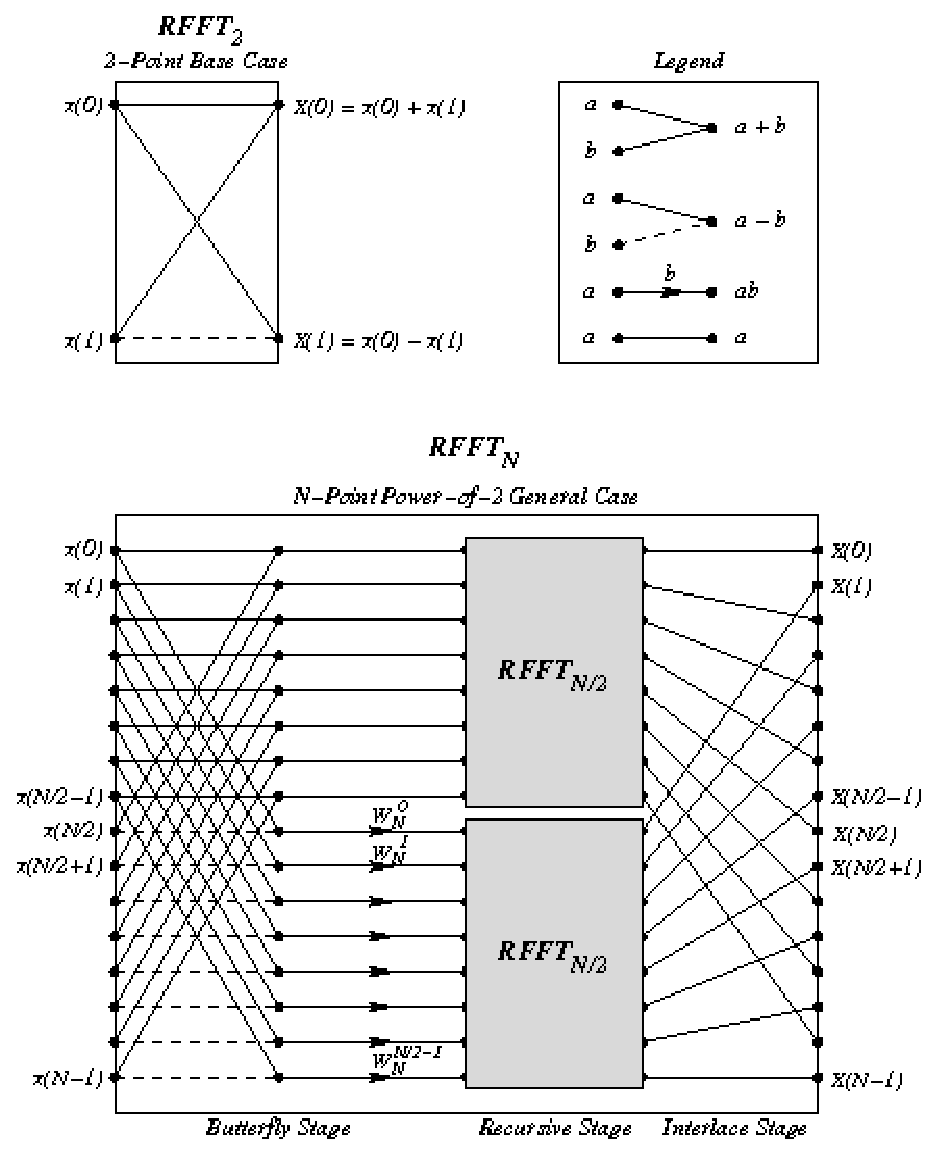
\includegraphics{math/45.eps}
\end{figure}



The diagram above is adapted from one by
Sam Daniel [\hyperref[bibliography_g225]{7}]
and shows the computational structure of the RFFT algorithm.
The first stage computes pairwise sums and differences
of the first and second halves of the input; this stage is labeled
the \textit{butterfly} stage.
The second stage recurs on the resulting subsequences.
The third stage interlaces the output of the
two recursive calls to RFFT, thus yielding the properly ordered
sequence \{\textit{X}(\textit{m})\}\textsubscript{\textit{m}=0}\textsuperscript{\textit{N}-1}.


The procedure \texttt{dft} accepts a sequence
(list) of values, \texttt{x}, the length of which
is assumed to be a power of 2.
\texttt{dft} precomputes a sequence of powers
of \(W_N\), \(\{W_N^n\}_{n=0}^{N/2-1}\), and calls \texttt{rfft} to
initiate the recursion.
\texttt{rfft} follows the algorithm outlined above.


\begin{alltt}
(define (dft x)
  (define (w-powers n)
    (let ([pi (* (acos 0.0) 2)])
      (let ([delta (/ (* -2.0i pi) n)])
        (let f ([n n] [x 0.0])
          (if (= n 0)
              '()
              (cons (exp x) (f (- n 2) (+ x delta))))))))
  (define (evens w)
    (if (null? w)
        '()
        (cons (car w) (evens (cddr w)))))
  (define (interlace x y)
    (if (null? x)
        '()
        (cons (car x) (cons (car y) (interlace (cdr x) (cdr y))))))
  (define (split ls)
    (let split ([fast ls] [slow ls])
      (if (null? fast)
          (values '() slow)
          (let-values ([(front back) (split (cddr fast) (cdr slow))])
            (values (cons (car slow) front) back)))))
  (define (butterfly x w)
    (let-values ([(front back) (split x)])
      (values
        (map + front back)
        (map * (map - front back) w))))
  (define (rfft x w)
    (if (null? (cddr x))
        (let ([x0 (car x)] [x1 (cadr x)])
          (list (+ x0 x1) (- x0 x1)))
        (let-values ([(front back) (butterfly x w)])
          (let ([w (evens w)])
            (interlace (rfft front w) (rfft back w))))))
  (rfft x (w-powers (length x))))
\end{alltt}

\paragraph{Exercise \label{examples_g199}12.9.1}


\label{examples_s71}Alter the algorithm to employ a base case of four points.
What simplifications can be made to avoid multiplying any of the
base case outputs by elements of \texttt{w}?


\paragraph{Exercise \label{examples_g200}12.9.2}


\label{examples_s72}Recode \texttt{dft} to accept a vector rather than a list as input, and
have it produce a vector as output.
Use lists internally if necessary, but do not simply convert the input to a
list on entry and the output to a vector on exit.


\paragraph{Exercise \label{examples_g201}12.9.3}


\label{examples_s73}Rather than recomputing the powers of \texttt{w} on each step for a new
number of points, the code simply uses the even-numbered elements of
the preceding list of powers.
Show that doing so yields the proper list of powers.
That is, show that \texttt{(evens (w-powers n))} is equal to
\texttt{(w-powers (/ n 2))}.


\paragraph{Exercise \label{examples_g202}12.9.4}


\label{examples_s74}The recursion step creates several intermediate lists that are
immediately discarded.
Recode the recursion step to avoid any unnecessary allocation.


\paragraph{Exercise \label{examples_g203}12.9.5}


\label{examples_s75}Each element of a sequence of input values may be regenerated from
the discrete Fourier transform of the sequence via the equation
\[X(n)=\frac{1}{N}\sum_{m=0}^{N-1}X(m)e^{i\frac{2\pi{}mn}{N}}\]
Noting the similarity between this equation and the original equation
defining \textit{X}(\textit{m}), create a modified version of \texttt{dft},
\texttt{inverse-dft}, that performs the inverse transformation.
Verify that \texttt{(inverse-dft (dft \textit{seq}))} returns
\texttt{\textit{seq}} for several input sequences \texttt{\textit{seq}}.

\section{\label{examples_g204}\label{examples_h10}A Unification Algorithm\label{examples_SECTEXUNIFY}}



\textit{Unification} [\hyperref[bibliography_g241]{23}] is a pattern-matching technique
used in automated theorem proving, type-inference systems, computer
algebra, and logic programming, e.g., Prolog [\hyperref[bibliography_g224]{6}].


A \label{examples_s76}unification algorithm attempts to make two symbolic expressions
equal by computing a unifying substitution for the expressions.
A \textit{substitution} is a function that replaces variables with other
expressions.
A substitution must treat all occurrences of a variable the same way,
e.g., if it replaces one occurrence of the variable \textit{x} by \textit{a}, it must
replace all occurrences of \textit{x} by \textit{a}.
A unifying substitution, or \textit{unifier}, for two expressions \textit{e}\textsubscript{1} and
\textit{e}\textsubscript{2} is a substitution, \(\sigma\), such that \(\sigma(e_1)=\sigma(e_2)\).


For example, the two expressions \textit{f}(\textit{x}) and \textit{f}(\textit{y}) can be unified by
substituting \textit{x} for \textit{y} (or \textit{y} for \textit{x}).
In this case, the unifier \(\sigma\) could be described as the function
that replaces \textit{y} with \textit{x} and leaves other variables unchanged.
On the other hand, the two expressions \textit{x} + 1 and \textit{y} + 2 cannot be
unified.
It might appear that substituting 3 for \textit{x} and 2 for \textit{y} would
make both expressions equal to 4 and hence equal to each other.
The symbolic expressions, 3 + 1 and 2 + 2, however, still differ.


Two expressions may have more than one unifier.
For example, the expressions \textit{f}(\textit{x},\textit{y}) and \textit{f}(1,\textit{y}) can be unified to
\textit{f}(1,\textit{y}) with the substitution of 1 for \textit{x}.
They may also be unified to \textit{f}(1,5) with the substitution of 1 for
\textit{x} and 5 for \textit{y}.
The first substitution is preferable, since it does not commit to
the unnecessary replacement of \textit{y}.
Unification algorithms typically produce the \textit{most general unifier},
or \textit{mgu}, for two expressions.
The mgu for two expressions makes no unnecessary substitutions; all
other unifiers for the expressions are special cases of the mgu.
In the example above, the first substitution is the mgu and the second
is a special case.


For the purposes of this program, a symbolic expression can be a variable,
a constant, or a function application.
Variables are represented by Scheme symbols, e.g., \texttt{x};
a function application is represented by a list with the function name in
the first position and its arguments in the remaining positions, e.g.,
\texttt{(f x)}; and
constants are represented by zero-argument functions, e.g., \texttt{(a)}.


The algorithm presented here finds the mgu for two terms, if it exists,
using a \label{examples_s77}continuation-passing style, or
CPS (see Section \ref{further_g75}),
approach to recursion on subterms.
The procedure \label{examples_s78}\texttt{unify} takes two terms and passes
them to a help procedure, \texttt{uni}, along with an initial (identity)
substitution, a success continuation, and a failure continuation.
The success continuation returns the result of applying its argument,
a substitution, to one of the terms, i.e., the unified result.
The failure continuation simply returns its argument, a message.
Because control passes by explicit continuation within \texttt{unify}
(always with tail calls), a return from the success or failure
continuation is a return from \texttt{unify} itself.


Substitutions are procedures.
Whenever a variable is to be replaced by another term, a new
substitution is formed from the variable, the term, and
the existing substitution.
Given a term as an argument, the new substitution replaces
occurrences of its saved variable with its saved term in the
result of invoking the saved substitution on the argument expression.
Intuitively, a substitution is a chain of procedures, one for each
variable in the substitution.
The chain is terminated by the initial, identity substitution.


\begin{alltt}
(unify 'x 'y) \(\Rightarrow\) y
(unify '(f x y) '(g x y)) \(\Rightarrow\) "clash"
(unify '(f x (h)) '(f (h) y)) \(\Rightarrow\) (f (h) (h))
(unify '(f (g x) y) '(f y x)) \(\Rightarrow\) "cycle"
(unify '(f (g x) y) '(f y (g x))) \(\Rightarrow\) (f (g x) (g x))
(unify '(f (g x) y) '(f y z)) \(\Rightarrow\) (f (g x) (g x))
\end{alltt}


\begin{alltt}
(library (tspl unification)
  (export unify)
  (import (rnrs))

 ; occurs? returns true if and only if u occurs in v
  (define occurs?
    (lambda (u v)
      (and (pair? v)
           (let f ([l (cdr v)])
             (and (pair? l)
                  (or (eq? u (car l))
                      (occurs? u (car l))
                      (f (cdr l))))))))

 ; sigma returns a new substitution procedure extending s by
 ; the substitution of u with v
  (define sigma
    (lambda (u v s)
      (lambda (x)
        (let f ([x (s x)])
          (if (symbol? x)
              (if (eq? x u) v x)
              (cons (car x) (map f (cdr x))))))))

 ; try-subst tries to substitute u for v but may require a
 ; full unification if (s u) is not a variable, and it may
 ; fail if it sees that u occurs in v.
  (define try-subst
    (lambda (u v s ks kf)
      (let ([u (s u)])
        (if (not (symbol? u))
            (uni u v s ks kf)
            (let ([v (s v)])
              (cond
                [(eq? u v) (ks s)]
                [(occurs? u v) (kf "cycle")]
                [else (ks (sigma u v s))]))))))

 ; uni attempts to unify u and v with a continuation-passing
 ; style that returns a substitution to the success argument
 ; ks or an error message to the failure argument kf.  The
 ; substitution itself is represented by a procedure from
 ; variables to terms.
  (define uni
    (lambda (u v s ks kf)

      (cond
        [(symbol? u) (try-subst u v s ks kf)]
        [(symbol? v) (try-subst v u s ks kf)]
        [(and (eq? (car u) (car v))
              (= (length u) (length v)))
         (let f ([u (cdr u)] [v (cdr v)] [s s])
           (if (null? u)
               (ks s)
               (uni (car u)
                    (car v)
                    s
                    (lambda (s) (f (cdr u) (cdr v) s))
                    kf)))]
        [else (kf "clash")])))

 ; unify shows one possible interface to uni, where the initial
 ; substitution is the identity procedure, the initial success
 ; continuation returns the unified term, and the initial failure
 ; continuation returns the error message.
  (define unify
    (lambda (u v)
      (uni u
           v
           (lambda (x) x)
           (lambda (s) (s u))
           (lambda (msg) msg)))))
\end{alltt}

\paragraph{Exercise \label{examples_g205}12.10.1}


\label{examples_s79}Modify \texttt{unify} so that it returns its substitution rather
than the unified term.
Apply this substitution to both input terms to verify that it
returns the same result for each.


\paragraph{Exercise \label{examples_g206}12.10.2}


\label{examples_s80}As mentioned above, substitutions on a term are performed
sequentially, requiring one entire pass through the input expression
for each substituted variable.
Represent the substitution differently so that only one pass
through the expression need be made.
Make sure that substitutions are performed not only on the input
expression but also on any expressions you insert during substitution.


\paragraph{Exercise \label{examples_g207}12.10.3}


\label{examples_s81}Extend the continuation-passing style unification algorithm into
an entire continuation-passing style logic programming system.



\section{\label{examples_g208}\label{examples_h11}Multitasking with Engines\label{examples_SECTEXENGINES}}



\label{examples_s82}Engines are a high-level process abstraction supporting
\label{examples_s83}\textit{timed
preemption} [\hyperref[bibliography_g228]{10},\hyperref[bibliography_g233]{15}].
Engines may be used to simulate \label{examples_s84}multiprocessing,
implement \label{examples_s85}\label{examples_s86}light-weight threads,
implement operating
system kernels, and perform \label{examples_s87}nondeterministic computations.
The engine implementation is one of the more interesting applications
of \label{examples_s88}continuations in Scheme.


An engine is created by passing a thunk (procedure of no arguments)
to the procedure \texttt{make-engine}.
The body of the thunk is the computation to be performed by the engine.
An engine itself is a procedure of three arguments:

\begin{enumerate}
\label{examples_g209}\item 
\label{examples_s89}\texttt{\textit{ticks}},
a positive integer that specifies the amount of \textit{fuel} to be given
to the engine.
An engine executes until this fuel runs out or until its computation
finishes.


\label{examples_g210}\item 
\label{examples_s90}\texttt{\textit{complete}},
a procedure of two arguments that
specifies what to do if the computation finishes.
Its arguments will be the amount of fuel left over and the
result of the computation.



\label{examples_g211}\item 
\label{examples_s91}\texttt{\textit{expire}},
a procedure of one argument that specifies what to do if the fuel runs
out before the computation finishes.
Its argument will be a new engine capable of continuing the computation
from the point of interruption.

\end{enumerate}


When an engine is applied to its arguments, it sets up a timer
to fire in \texttt{\textit{ticks}} time units.
If the engine computation completes before the timer goes off, the
system invokes \texttt{\textit{complete}}, passing it the
number of \texttt{\textit{ticks}} left over
and the value of the computation.
If, on the other hand, the timer goes off before the engine computation
completes, the system creates a new engine from the continuation of
the interrupted computation and passes this engine to \texttt{\textit{expire}}.
\texttt{\textit{complete}} and \texttt{\textit{expire}} are invoked in the continuation
of the engine invocation.


The following example creates an engine from a trivial computation,
3, and gives the engine 10 ticks.


\begin{alltt}
(define eng
  (make-engine
    (lambda () 3)))

(eng 10
  (lambda (ticks value) value)
  (lambda (x) x)) \(\Rightarrow\) 3
\end{alltt}


It is often useful to pass \texttt{list} as the \texttt{\textit{complete}} procedure
to an engine, causing the engine to return a list of the
ticks remaining and the value if the computation completes.


\begin{alltt}
(eng 10
  list
  (lambda (x) x)) \(\Rightarrow\) (9 3)
\end{alltt}


In the example above, the value was 3 and there were 9 ticks left over,
i.e., it took only one unit of fuel to evaluate 3.
(The fuel amounts given here are for illustration only.
The actual amount may differ.)


Typically, the engine computation does not finish in one try.
\label{examples_s92}The following example displays the use of an engine to
compute the 10th Fibonacci number (see Section \ref{further_g55})
in steps.


\begin{alltt}
(define fibonacci
  (lambda (n)
    (if (\textless{} n 2)
        n
        (+ (fibonacci (- n 1))
           (fibonacci (- n 2))))))

(define eng
  (make-engine
    (lambda ()
      (fibonacci 10))))

(eng 50
  list
  (lambda (new-eng)
    (set! eng new-eng)
    "expired")) \(\Rightarrow\) "expired"

(eng 50
  list
  (lambda (new-eng)
    (set! eng new-eng)
    "expired")) \(\Rightarrow\) "expired"

(eng 50
  list
  (lambda (new-eng)
    (set! eng new-eng)
    "expired")) \(\Rightarrow\) "expired"

(eng 50
  list
  (lambda (new-eng)
    (set! eng new-eng)
    "expired")) \(\Rightarrow\) (22 55)
\end{alltt}


Each time the engine's fuel ran out, the \texttt{\textit{expire}} procedure assigned
\texttt{eng} to the new engine.
The entire computation required four allotments of 50 ticks to complete; of the
last 50 it used all but 23.
Thus, the total amount of fuel used was 177 ticks.
This leads us to the following procedure, \texttt{mileage}, which
uses engines to ``time'' a computation.


\begin{alltt}
(define mileage
  (lambda (thunk)
    (let loop ([eng (make-engine thunk)] [total-ticks 0])
      (eng 50
        (lambda (ticks value)
          (+ total-ticks (- 50 ticks)))
        (lambda (new-eng)
          (loop new-eng (+ total-ticks 50)))))))

(mileage (lambda () (fibonacci 10))) \(\Rightarrow\) 178
\end{alltt}


The choice of 50 for the number of ticks to use each time is
arbitrary, of course.
It might make more sense to pass a much larger number, say 10000,
in order to reduce the number of times the computation is interrupted.


The next procedure, \label{examples_s93}\texttt{round-robin}, could be the basis for a simple
time-sharing \label{examples_s94}operating system.
\texttt{round-robin} maintains a queue of processes (a list of engines)
and cycles through the queue in a \textit{round-robin} fashion, allowing each
process to run for a set amount of time.
\texttt{round-robin} returns a list of the values returned by the engine
computations in the order that the computations complete.


\begin{alltt}
(define round-robin
  (lambda (engs)
    (if (null? engs)
        '()
        ((car engs) 1
          (lambda (ticks value)
            (cons value (round-robin (cdr engs))))
          (lambda (eng)
            (round-robin
              (append (cdr engs) (list eng))))))))
\end{alltt}


Assuming the amount of computation corresponding to one tick is constant,
the effect of \texttt{round-robin} is to return a list of the values sorted
from the quickest to complete to the slowest to complete.
Thus, when we call \texttt{round-robin} on a list of engines, each computing
one of the Fibonacci numbers, the output list is sorted with the earlier
Fibonacci numbers first, regardless of the order of the input list.


\begin{alltt}
(round-robin
  (map (lambda (x)
         (make-engine
           (lambda ()
              (fibonacci x))))
       '(4 5 2 8 3 7 6 2))) \(\Rightarrow\) (1 1 2 3 5 8 13 21)
\end{alltt}


More interesting things could happen if the amount of fuel varied
each time through the loop.
\label{examples_s95}In this case, the computation would
be nondeterministic, i.e., the results would vary from call to call.


The following syntactic form, \label{examples_s96}\texttt{por} (parallel-or), returns the
first of its expressions to complete with a true value.
\texttt{por} is implemented with the procedure \texttt{first-true}, which is
similar to \texttt{round-robin} but quits when any of the engines
completes with a true value.
If all of the engines complete, but none with a true value,
\texttt{first-true} (and hence \texttt{por}) returns \texttt{\#{}f}.


\begin{alltt}
(define-syntax por
  (syntax-rules ()
    [(\_{} x ...)
     (first-true
       (list (make-engine (lambda () x)) ...))]))

(define first-true
  (lambda (engs)
    (if (null? engs)
        \#{}f
        ((car engs) 1
          (lambda (ticks value)
            (or value (first-true (cdr engs))))
          (lambda (eng)
            (first-true
              (append (cdr engs) (list eng))))))))
\end{alltt}


Even if one of the expressions is an infinite loop,
\texttt{por} can still finish (as long as one of the other expressions
completes and returns a true value).


\begin{alltt}
(por 1 2) \(\Rightarrow\) 1
(por ((lambda (x) (x x)) (lambda (x) (x x)))
     (fibonacci 10)) \(\Rightarrow\) 55
\end{alltt}


The first subexpression of the second \texttt{por} expression is
nonterminating, so the answer is the value of the second
subexpression.


Let's turn to the implementation of engines.
Any preemptive multitasking primitive must have the ability to
interrupt a running process after a given amount of computation.
This ability is provided by a primitive \label{examples_s97}timer
interrupt mechanism in some Scheme implementations.
We will construct a suitable one here.


Our timer system defines three procedures: \texttt{start-timer}, \texttt{stop-timer},
and \texttt{decrement-timer}, which can be described operationally as
follows.

\begin{itemize}
\item 
\texttt{(start-timer \textit{ticks} \textit{handler})}
sets the timer
to \texttt{\textit{ticks}} and installs \texttt{\textit{handler}} as the procedure to be
invoked (without arguments) when the timer expires, i.e., reaches zero.

\item 
\texttt{(stop-timer)}
resets the timer and returns the number of ticks remaining.

\item 
\texttt{(decrement-timer)}
decrements the timer by one tick if the timer is on, i.e., if it is
not zero.
When the timer reaches zero, \texttt{decrement-timer} invokes the saved
handler.
If the timer has already reached zero, \texttt{decrement-timer} returns
without changing the timer.

\end{itemize}


Code to implement these procedures is given along with the engine
implementation below.


Using the timer system requires inserting calls to \texttt{decrement-timer} in
appropriate places.
Consuming a timer tick on entry to a procedure usually provides a sufficient
level of granularity.
This can be accomplished by using \texttt{timed-lambda} as defined below
in place of \texttt{lambda}.
\texttt{timed-lambda} simply invokes \texttt{decrement-timer} before executing the
expressions in its body.


\begin{alltt}
(define-syntax timed-lambda
  (syntax-rules ()
    [(\_{} formals exp1 exp2 ...)
     (lambda formals (decrement-timer) exp1 exp2 ...)]))
\end{alltt}


It may be useful to redefine named \texttt{let} and \texttt{do} to use \texttt{timed-lambda}
as well, so that recursions expressed with these constructs are
timed.
If you use this mechanism, do not forget to use the timed versions of
\texttt{lambda} and other forms in code run within an engine, or no
ticks will be consumed.


Now that we have a suitable timer, we can implement engines in terms of
the timer and continuations.
We use \label{examples_s98}\texttt{call/cc} in two places in the engine
implementation: (1) to obtain the continuation of the computation that invokes
the engine so that we can return to that continuation when the engine
computation completes or the timer expires, and (2) to obtain the continuation
of the engine computation when the timer expires so that we can return
to this computation if the newly created engine is subsequently run.


The state of the engine system is contained in two variables local to
the engine system: \texttt{do-complete} and \texttt{do-expire}.
When an engine is started, the engine assigns to \texttt{do-complete} and
\texttt{do-expire} procedures
that, when invoked, return to the continuation of the engine's caller
to invoke \texttt{\textit{complete}} or \texttt{\textit{expire}}.
The engine starts (or restarts) the computation by invoking
the procedure passed as an argument to \texttt{make-engine} with the specified
number of ticks.
The ticks and the local procedure \texttt{timer-handler} are then used to
start the timer.


Suppose that the timer expires before the engine computation completes.
The procedure \texttt{timer-handler} is then invoked.
It initiates a call to \texttt{start-timer} but obtains the ticks by calling
\texttt{call/cc} with \texttt{do-expire}.
Consequently, \texttt{do-expire} is
called with a continuation that, if invoked,
will restart the timer and continue the interrupted computation.
\texttt{do-expire} creates a new engine from this continuation and
arranges for the engine's \texttt{\textit{expire}} procedure to be invoked with the new
engine in the correct continuation.


If, on the other hand, the engine computation completes before
the timer expires, the timer is stopped and the number of ticks remaining
is passed along with the value to \texttt{do-complete};
\texttt{do-complete} arranges for the engine's \texttt{\textit{complete}} procedure
to be invoked with the ticks and value in the correct continuation.


Let's discuss a couple of subtle aspects to this code.
The first concerns the method used to start the timer when an engine
is invoked.
The code would apparently be simplified by letting \texttt{new-engine} start
the timer before it initiates or resumes the engine computation, instead
of passing the ticks to the computation and letting it start the timer.
Starting the timer within the computation, however, prevents ticks from
being consumed prematurely.
If the engine system itself consumes fuel, then an engine provided with a
small amount of fuel may not progress toward completion.
(It may, in fact, make negative progress.)
If the software timer described above is used, this problem is actually
avoided by compiling the engine-making code with the untimed version of
\texttt{lambda}.


The second subtlety concerns the procedures created by \texttt{do-complete} and
\texttt{do-expire} and subsequently applied by the continuation of the
\label{examples_s99}\label{examples_s100}\texttt{call/cc} application.
It may appear that \texttt{do-complete} could first invoke the engine's
\texttt{\textit{complete}} procedure, then pass the result to the continuation
(and similarly for \texttt{do-expire}) as follows.


\texttt{(escape (complete value ticks))}

This would result in improper treatment of tail recursion, however.
The problem is that the current continuation would not be replaced with the
continuation stored in \texttt{escape} until the call to the \texttt{complete}
procedure returns.
Consequently, both the continuation of the running engine and the continuation
of the engine invocation could be retained for an indefinite period of time,
when in fact the actual engine invocation may appear to be tail-recursive.
This is especially inappropriate because the engine interface encourages use of
continuation-passing style and hence tail recursion.
The round-robin scheduler and \texttt{first-true} provide good examples of this,
since the \texttt{\textit{expire}} procedure in each invokes engines tail-recursively.


We maintain proper treatment of tail recursion by arranging for
\texttt{do-complete} and \texttt{do-expire} to escape from
the continuation of the running engine before invoking the \texttt{complete} or
\texttt{expire} procedures.
Since the continuation of the engine invocation is a procedure application,
passing it a procedure of no arguments results in application of the procedure
in the continuation of the engine invocation.


\begin{alltt}
(library (tspl timer)
  (export start-timer stop-timer decrement-timer)
  (import (rnrs))

  (define clock 0)
  (define handler \#{}f)

  (define start-timer
    (lambda (ticks new-handler)
      (set! handler new-handler)
      (set! clock ticks)))

  (define stop-timer
    (lambda ()
      (let ([time-left clock])
        (set! clock 0)
        time-left)))

  (define decrement-timer
    (lambda ()
      (when (\textgreater{} clock 0)
        (set! clock (- clock 1))
        (when (= clock 0) (handler)))))

  (define-syntax timed-lambda
    (syntax-rules ()
      [(\_{} formals exp1 exp2 ...)
       (lambda formals (decrement-timer) exp1 exp2 ...)])))

(library (tspl engines)
  (export make-engine timed-lambda)
  (import (rnrs) (tspl timer))

  (define make-engine
    (let ([do-complete \#{}f] [do-expire \#{}f])
      (define timer-handler
        (lambda ()
          (start-timer (call/cc do-expire) timer-handler)))
      (define new-engine
        (lambda (resume)
          (lambda (ticks complete expire)
            ((call/cc
               (lambda (escape)
                 (set! do-complete
                   (lambda (ticks value)
                     (escape (lambda () (complete ticks value)))))
                 (set! do-expire
                   (lambda (resume)
                     (escape (lambda ()
                               (expire (new-engine resume))))))
                 (resume ticks)))))))
      (lambda (proc)
        (new-engine
          (lambda (ticks)
            (start-timer ticks timer-handler)
            (let ([value (proc)])
              (let ([ticks (stop-timer)])
                (do-complete ticks value))))))))

  (define-syntax timed-lambda
    (syntax-rules ()
      [(\_{} formals exp1 exp2 ...)
       (lambda formals (decrement-timer) exp1 exp2 ...)])))
\end{alltt}

\paragraph{Exercise \label{examples_g212}12.11.1}


\label{examples_s101}If your Scheme implementation allows definition and import of libraries
in the interactive top level, try defining the libraries above, then
type


\texttt{(import (rename (tspl engines) (timed-lambda lambda)))}

to define \texttt{make-engine} and redefine \texttt{lambda}.
Then try out the examples given earlier in this section.


\paragraph{Exercise \label{examples_g213}12.11.2}


\label{examples_s102}It may appear that the nested \texttt{let} expressions in the body of
\texttt{make-engine}:


\begin{alltt}
(let ([value (proc)])
  (let ([ticks (stop-timer)])
    (do-complete ticks value)))
\end{alltt}


could be replaced with the following.


\begin{alltt}
(let ([value (proc)] [ticks (stop-timer)])
  (do-complete value ticks))
\end{alltt}


Why is this not correct?


\paragraph{Exercise \label{examples_g214}12.11.3}


\label{examples_s103}It would also be incorrect to replace the
nested \texttt{let} expressions discussed in the preceding exercise
with the following.


\begin{alltt}
(let ([value (proc)])
  (do-complete value (stop-timer)))
\end{alltt}


Why?


\paragraph{Exercise \label{examples_g215}12.11.4}


\label{examples_s104}Modify the engine implementation to provide a procedure,
\texttt{engine-return}, that returns immediately from an engine.


\paragraph{Exercise \label{examples_g216}12.11.5}


\label{examples_s105}Implement the kernel of a small \label{examples_s106}operating
system using engines for processes.
Processes should request services (such as reading input from the user)
by evaluating an expression of the form \texttt{(trap 'request)}.
Use \texttt{call/cc} and \texttt{engine-return} from the preceding
exercise to implement \texttt{trap}.


\paragraph{Exercise \label{examples_g217}12.11.6}


\label{examples_s107}Write the same operating-system kernel without using engines, building
instead from continuations and timer interrupts.


\paragraph{Exercise \label{examples_g218}12.11.7}


\label{examples_s108}This implementation of engines does not allow one engine to call
another, i.e., nested engines [\hyperref[bibliography_g228]{10}].
Modify the implementation to allow \label{examples_s109}nested
engines.



